%%%%%%%%%%%%%%%%%%%%%%%%%%%%%%%%%%%%%%%%%%%%%%%%%%%%%%%%%%%%%%%%%%%%%%
% Lớp 12 | Ứng dụng đạo hàm để khảo sát hàm số | Đường tiệm cận
% Dạng 2D1?4-1: Bài toán xác định các đường tiệm cận của hàm số (không chứa tham số )
% Số câu: 108  (sinh tự động bởi tach_cau.py; từ nay thầy sửa trực tiếp file này)
%%%%%%%%%%%%%%%%%%%%%%%%%%%%%%%%%%%%%%%%%%%%%%%%%%%%%%%%%%%%%%%%%%%%%%

%%%%%%%%%%%%%%%% TRẮC NGHIỆM 4 PHƯƠNG ÁN %%%%%%%%%%%%%%%%

% nguồn: Phan1_Lop_12_Dai_so_Chuong_1
\begin{ex}%[2D1N4-1]%[ma:288a9065]
	Đường tiệm cận đứng của đồ thị hàm số  $y=\dfrac{x^2+x-2}{x-2}$ là
	 \choice
		{\True  $x=2$}
		{$x=-2$} 
		{$y=-2$} 
		{$y=2$} 
	 \loigiai{
	Tập xác định: $D=\mathbb{R} \backslash\{2\}$ và $\lim\limits_{x \rightarrow 2^{+}} \dfrac{x^{2}+x-2}{x-2}=+\infty$.\\ $\Rightarrow$ Tiệm cận đứng là  $x=2$.}
\end{ex}

% nguồn: Phan1_Lop_12_Dai_so_Chuong_1
\begin{ex}%[2D1N4-1]%[ma:f27cf721]
	Cho hàm số $y=f(x)$ xác định và liên tục  trên $\mathbb{R} \setminus\{-1\}$, có bảng biến thiên như sau.
	\begin{center}
		
\begin{tikzpicture}[scale=1,font=\footnotesize,line join=round,line cap=round,>=stealth]
			 \tkzTabInit[espcl=3,lgt=1.5]
				 {$x$/0.7,$y'$/0.7,$y$/2.1}
				 {$-\infty$,$-1$,$+\infty$}
			 \tkzTabLine{,+,d,+,}
			 \tkzTabVar{-/$-2$,+D-/$+\infty$/$-\infty$,+/$-2$}
		\end{tikzpicture}
	\end{center}
	Khẳng định nào sau đây  là đúng?
	 \choice
		{Đồ thị  hàm số có tiệm cận đứng $y=-1$ và tiệm cận ngang $x=-2$}
		{Đồ thị hàm  số có duy nhất một tiệm cận}
		{Đồ thị hàm  số có ba tiệm cận}
		{\True Đồ thị hàm  số có tiệm cận đứng $x=-1$ và tiệm cận ngang $y=-2$}
	 \loigiai{
		Từ bảng biến thiên suy ra $\lim\limits_{x \rightarrow+\infty} y=-2$.\\ Do đó đồ thị hàm số  có tiệm cận ngang $y=-2$.\\
	Mặt khác $\lim\limits_{x \rightarrow(-1)^-}y=+\infty$ nên  đồ thị hàm số có tiệm cận đứng $x=-1$.}
\end{ex}

% nguồn: Phan1_Lop_12_Dai_so_Chuong_1
\begin{ex}%[2D1N4-1]%[ma:cbb95981]
	Tiệm cận ngang của đồ thị hàm số $y=\dfrac{2}{x-1}$  là đường thẳng
	\choice 
		 {$x=1$}
		 {$y=2$}
		 {$x=0$}
		{\True $y=0$} 
	 \loigiai{
	Ta có $\lim\limits_{x \rightarrow+\infty} \dfrac{2}{x-1}=0; \lim\limits_{x \rightarrow-\infty} \dfrac{2}{x-1}=0$. \\Vậy đường thẳng $y=0$ là tiệm cận  ngang của đồ thị hàm số.}
\end{ex}

% nguồn: Phan1_Lop_12_Dai_so_Chuong_1
\begin{ex}%[2D1N4-1]%[ma:f16262ea]
	Phương trình đường tiệm cận đứng của đồ thị  hàm số $y=\dfrac{3}{x+2}$ là
	 \choice
		{\True  $x=-2$}
		 {$x=0$}
		 {$x=3$}
		{$y=0$} 
	\loigiai{ 
		Tập xác đinh  $\mathscr{D}=\mathbb{R} \setminus\{-2\}$.
		\begin{itemize}
			\item $\lim\limits_{x \rightarrow-2^{+}} y=\lim\limits_{x \rightarrow-2^{+}} \dfrac{3}{x+2}=+\infty$. 
			 \item $\lim\limits_{x \rightarrow-2^-} y=\lim\limits_{x \rightarrow-2^-} \dfrac{3}{x+2}=-\infty$.
		\end{itemize}
	Suy ra $x=-2$ là tiệm cận đứng của  đồ thị hàm số.}
\end{ex}

% nguồn: Phan1_Lop_12_Dai_so_Chuong_1
\begin{ex}%[2D1N4-1]%[ma:a77bf496]
	Đồ thị hàm số $y=\dfrac{x-2}{x^{2}-4}$ có đường tiệm cận ngang  là
	\choice 
		 {$y=2$}
		{\True $y=0$} 
		{$y=1$} 
		{$y=-2$} 
	 \loigiai{
		Tập xác  định $\mathscr{D}=\mathbb{R} \setminus\{\pm 2\}$.\\
	Ta có $\lim\limits_{x \rightarrow \pm \infty} \dfrac{x-2}{x^{2}-4}=0$ suy ra đồ thị hàm  số có đường tiệm cận ngang là $y=0$.}
\end{ex}

% nguồn: Phan1_Lop_12_Dai_so_Chuong_1
\begin{ex}%[2D1N4-1]%[ma:6f9ef469]
	Cho hàm số $y=f(x)$ xác định và liên tục trên $(-\infty;0)$ và $(0;+\infty)$ có bảng biến thiên như hình vẽ.  Mệnh đề nào sau đây \textbf{đúng}?
	\begin{center}
		
\begin{tikzpicture}[scale=1,font=\footnotesize,line join=round,line cap=round,>=stealth]
			\tkzTabInit[espcl=3,lgt=1.5] 
				{$x$/0.7,$f'(x)$/0.7,$f  (x)$/2.1}
				 {$-\infty$,$0$,$3$,$+\infty$}
			\tkzTabLine{,-,d,-,0,+,} 
			 \tkzTabVar{+/$1$,-D+/$-\infty$/$+\infty$,-/$2$,+/$+\infty$}
		\end{tikzpicture}
	\end{center}
	\choice 
		{Đường thẳng  $x=2$ là tiệm cận đứng của đồ thị hàm số}
		{Đồ  thị hàm số có hai đường tiệm cận ngang}
		{\True Đồ thị hàm số  có hai đường tiệm cận}
		{Đồ thị hàm số chỉ có một đường tiệm cận} 
	 \loigiai{
		Vì $\lim\limits_{x\rightarrow-\infty}y=2$ nên $y=2$ là tiệm cận ngang của  đồ thị hàm số.\\
		Vì $\heva{&\lim\limits_{x \rightarrow 0^+} y=+\infty\\&\lim\limits_{x \rightarrow 0^-}y=-\infty}$ nên $x=0$ là tiệm cận  đứng của đồ thị hàm số.\\
	 Vậy đồ thị hàm số có $2$ đường tiệm cận.}
\end{ex}

% nguồn: Phan1_Lop_12_Dai_so_Chuong_1
\begin{ex}%[2D1N4-1]%[ma:3c351e5e]
	\immini{Cho hàm số $f(x)$ có đồ thị như hình bên. Biết rằng  một trong bốn điểm sau đây là tâm đối xứng của đồ thị hàm số, điểm đó là điểm nào?
	 \choice
		 {$M(0;1)$}
		{\True  $N(-1;2)$}
		{$P(-2;3)$} 
		 {$Q(0;3)$}
		}{\resizebox{!}{5cm}{\begin{tikzpicture}[line join=round,line cap=round,>=stealth]
		 \tikzset{label style/.style={font=\footnotesize}}
		 \draw[->] (-4.1,0)--(3.1,0) node[below left] {$x$};
		\draw[->] (0,-2.1)--(0,5.1) node[below  left] {$y$};
		\draw (0,0)  node [below left] {$O$};
		\foreach \x  in {-3,-2,-1,1,2}
		\draw (\x,1pt)--(\x,-1pt) node [below]  {$\x$};
		\foreach  \y in {-2,-1,1,2,3,4}
		\draw (1pt,\y)--(-1pt,\y) node [left] {$\y$}; 
		\begin{scope}
			\clip  (-4,-2) rectangle (3,5);
			\draw[samples=100,domain=-4:-1.01,smooth,variable=\x] plot  (\x,{(2*(\x)+1)/((\x)+1)});
			 \draw[samples=100,domain=-0.99:3,smooth,variable=\x] plot (\x,{(2*(\x)+1)/((\x)+1)});
		\end{scope}
	\end{tikzpicture}
		 }}
	\loigiai{Đồ thị hàm số có tiệm cận đứng $x=-1$, và tiệm cận ngang là  $y=2$ nên tâm đối xứng là $N\left(-1;2\right)$.}
\end{ex}

% nguồn: Phan1_Lop_12_Dai_so_Chuong_1
\begin{ex}%[2D1N4-1]%[ma:454844fe]
	\immini{Cho hàm số $f(x)$ có đồ thị như hình bên. Biết rằng một trong bốn đường thẳng sau đây là đường tiệm cận  xiên của đồ thị hàm số, đường đó là đường nào?
	\choice 
		 {$y=2x$}
		{$y=\dfrac{-x}{2}$} 
		{\True  $y=-2x$}
		{$y=\dfrac{x}{2}$} 
		}{\resizebox{!}{5cm}{\begin{tikzpicture}
		 \draw[->] (-3.1,0)--(3.1,0) node[below left] {$x$};
		\draw[->] (0,-3.1)--(0,4.1) node[below  left] {$y$};
		\draw (0,0) node [below left] {$O$}; 
		\foreach \x  in {-2,-1,1,2}
		\draw (\x,1pt)--(\x,-1pt) node  [below] {$\x$};
		\foreach \y  in {-2,-1,1,2}
		\draw (1pt,\y)--(-1pt,\y)  node [left] {$\y$};
		\begin{scope}
			\clip (-3,-3) rectangle (3,4); 
			\draw[samples=100,domain=-3:-0.01,smooth,variable=\x] plot  (\x,{(-2*((\x)^2)+0*(\x)+1)/((\x)+0)});
			 \draw[samples=100,domain=0.01:3,smooth,variable=\x] plot (\x,{(-2*((\x)^2)+0*(\x)+1)/((\x)+0)});
			 \draw (-3.1,6.2)--(3.1,-6.2);
		\end{scope}
	\end{tikzpicture}
		 }}
	\loigiai{ 
		Gọi tiệm cận xiên của đồ thị có dạng  $d \colon y=ax+b$ ($a\ne 0$).\\
		Mà $\heva{&O(0;0) \in  d\\& A(-1;2)\in d} \Rightarrow \heva{&0=b\\&2=-a+b} \Rightarrow \heva{&a=-2\\&b=0}$.\\
	Nên tiệm cận xiên của đồ thị hàm  số là $d\colon y=-2x$.}
\end{ex}

% nguồn: Phan1_Lop_12_Dai_so_Chuong_1
\begin{ex}%[2D1N4-1]%[ma:0b4695b1]
	Cho hàm số $y=f(x)$ có  bảng biến thiên như sau.
	\begin{center}
		
\begin{tikzpicture}[scale=0.9,>=stealth]
			 \tkzTabInit[nocadre=false,lgt=2,espcl=2.7,deltacl=0.6]
				 {$x$/0.8,$f'(x)$/0.8,$f (x)$/3}
				 {$-\infty$,$-1$,$2$,$+\infty$}
			\tkzTabLine{,-,0,+,d,+,} 
			\tkzTabVar{+/$0$,-/$1$,+D-/$+\infty$/$-2$,+/$+\infty$} 
		\end{tikzpicture}
	\end{center}
	Tổng số tiệm cận ngang và tiệm cận đứng của đồ  thị hàm số $y=f(x)$ là
	 \choice
		{\True  $2$}
		{$4$} 
		 {$3$}
		 {$1$}
	\loigiai{ 
		Ta có $\lim_{x\to +\infty}  y=+\infty$.\\
		$\lim_{x\to -\infty} y=0 \Rightarrow y=0$  là một tiệm cận ngang của đồ thị hàm số.\\
		$\lim_{x\to 2^{-}} y=+\infty \Rightarrow x=2$ là một tiệm cận  đứng của đồ thị hàm số.
	 }
\end{ex}

% nguồn: Phan1_Lop_12_Dai_so_Chuong_1
\begin{ex}%[2D1N4-1]%[ma:ee390dab]
	Cho hàm số $y=f(x)$ có  bảng biến thiên sau
	\begin{center}
		
\begin{tikzpicture}[scale=1,line join=round,line cap=round,font=\footnotesize,>=stealth]
			 \tkzTabInit[nocadre=false,lgt=2,espcl=3,deltacl=1]
				 {$x$/0.7,$f’(x)$/0.7,$f (x)$/2}
				{$-\infty$,$0$,$2$,$+\infty$} 
			\tkzTabLine{,-,d,+,d,-,} 
			\tkzTabVar{+/$2$,-D-/$-\infty$,+D+/$+\infty$,-/$-2$} 
		\end{tikzpicture}
	\end{center}
	Tổng số tiệm cận đứng và tiệm cận  ngang của đồ thị hàm số đã cho là
	\choice 
		 {$1$}
		{$2$} 
		 {$3$}
		{\True  $4$}
	 \loigiai{
		Đồ thị hàm số $y=f(x)$ có hai tiệm cận  đứng là $x=0$, $x=2$ và hai tiệm cận ngang là $y=2$, $y=-2$.\\
		Vậy  có $4$ tiệm cận.
	 }
\end{ex}

% nguồn: Phan1_Lop_12_Dai_so_Chuong_1
\begin{ex}%[2D1N4-1]%[ma:45117567]
	Đồ thị của hàm số nào  dưới đây có tiệm cận ngang?
	\choice 
		 {$y=x^3-x-1$}
		 {$y=\sqrt{2x^2+3}$}
		 {$y=\dfrac{x^3+1}{x^2+1}$}
		{\True  $y=\dfrac{3x^2+2x-1}{4x^2+5}$}
	\loigiai{ 
		Ta có $\lim\limits_{x \rightarrow+\infty} y=\lim\limits_{x  \rightarrow+\infty} \dfrac{3 x^2+2 x+1}{4 x^2+5}=\dfrac{3}{4}$. \\
	Suy ra đồ thị hàm số có tiệm cận ngang $y=\dfrac{3}{4}$.} 
\end{ex}

% nguồn: Phan1_Lop_12_Dai_so_Chuong_1
\begin{ex}%[2D1N4-1]%[ma:f5665ad2]
	 \immini{
	Cho hàm số $f(x)=\dfrac{ax+b}{cx+d}$ ($a$, $b$, $c$, $d\in \mathbb{R}$, $c\neq 0$) có đồ thị  như hình bên. Đường tiệm cận đứng của đồ thị hàm số là
	 \choice
		{$y=-2$} 
		 {$y=2$}
		 {$x=-2$}
		{\True $x=2$} 
		} 
		{ 
		\begin{tikzpicture}[scale=0.4,font=\footnotesize,line join=round,line cap=round,>=stealth]
			\draw[->] (-6.1,0)--(8.1,0) node[below left] {$x$}; 
			\draw[->] (0,-7.1)--(0,7.1) node[below  left] {$y$};
			\draw (0,0) node [below left] {$O$} circle (1pt); 
			\draw (2,0) node [below left] {$2$} circle (1pt); 
			 \draw (-2,0) node [below] {$-2$} circle (1pt);
			 \draw (0,2) node [right] {$2$} circle (1pt);
			\draw (0,-2) node [right] {$-2$} circle (1pt); 
			 \draw[dashed] (2.01,-7)--(2.01,7);
			\begin{scope}
				\clip  (-7,-7) rectangle (8,7);
				\draw[samples=100,domain=-6:1.9,smooth,variable=\x] plot (\x,{(0*(\x)+6)/((\x)+-2)}); 
				\draw[samples=100,domain=2.1:8,smooth,variable=\x]  plot (\x,{(0*(\x)+6)/((\x)+-2)});
				 \draw (-6,0/1)--(6,0/1);
			\end{scope}
		\end{tikzpicture}
		} 
	 \loigiai{
		Từ  đồ thị suy ra đường tiệm cận đứng là $x=2$.
	 }
\end{ex}

% nguồn: Phan1_Lop_12_Dai_so_Chuong_1
\begin{ex}%[2D1N4-1]%[ma:401e8b75]
	Đường tiệm cận  của đồ thị hàm số $y=\dfrac{1}{x^{2}+1}$ có phương trình
	 \choice
		{$y=2$} 
		{$y=3$} 
		 {$y=1$}
		{\True  $y=0$}
	 \loigiai{
		Tập xác  định: $\mathscr{D}=\mathbb{R}$.\\
	Ta có $\lim\limits_{x \rightarrow \pm \infty} y=0$ nên $y=0$ là đường tiệm  cận ngang của đồ thị hàm số.}
\end{ex}

% nguồn: Phan1_Lop_12_Dai_so_Chuong_1
\begin{ex}%[2D1N4-1]%[ma:548414cd]
	 Xét hàm số $y=f(x)$ có bảng biến thiên như sau
	\begin{center}
		
\begin{tikzpicture}[scale=1,font=\footnotesize,line join=round,line cap=round,>=stealth]
			 \tkzTabInit[nocadre=true,lgt=1,espcl=3,deltacl=0.5]
				{$x$/.7,$y'$/.7,$y$/2} 
				 {$-\infty$,$1$,$+\infty$}
			\tkzTabLine{,-,d,-,} 
			\tkzTabVar{+/$2$,-D+/$-\infty$/$+\infty$,-/$2$} 
		\end{tikzpicture}
	\end{center}
	 Mệnh đề nào dưới đây đúng?
	 \choice
		{Đồ thị hàm số có tiệm  cận ngang là đường thẳng $x=1$ và tiệm cận đứng là đường thẳng $y=2$}
		{Đồ thị hàm số không có  đường tiệm cận}
		{\True Đồ thị hàm số có tiệm  cận đứng là đường thẳng $x=1$ và đường tiệm cận ngang là đường thẳng $y=2$}
		{Đồ thị  hàm số chỉ có một đường tiệm cận}
	 \loigiai{
		Từ  bảng biến thiên, ta có
		\begin{itemize}
			\item $\lim\limits_{x\to +\infty}y=2$ và $\lim\limits_{x\to -\infty}y=2$.\\ 
			Suy ra đường tiệm cận ngang của đồ thị hàm số là  đường thẳng $y=2$.
			\item $\lim\limits_{x\to  1^+}y=+\infty $và $\lim\limits_{x\to 1^-}y=-\infty$.\\
			Suy ra đường tiệm cận đứng của  đồ thị hàm số là đường thẳng $x=1$.
		\end{itemize}
	 }
\end{ex}

% nguồn: Phan1_Lop_12_Dai_so_Chuong_1
\begin{ex}%[2D1N4-1]%[ma:796f3add]
	Tiệm cận ngang của đồ thị hàm số $y=\dfrac{3x-1}{x+1}$ là  đường thẳng
	\choice 
		 {$x=3$}
		{\True $y=3$} 
		{$x=-1$} 
		{$y=-1$} 
	\loigiai{ 
		Ta có\\ 
		$\lim_{x\to +\infty}  \dfrac{3x-1}{x+1}=3$.\\
		$\lim_{x\to -\infty}  \dfrac{3x-1}{x+1}=3$.\\
		Vậy đường thẳng $y=3$ là tiệm cận ngang của đồ thị hàm số. 
	 }
\end{ex}

% nguồn: Phan1_Lop_12_Dai_so_Chuong_1
\begin{ex}%[2D1N4-1]%[ma:e4ecb4d2]
	Cho hàm số $y=f(x)$ xác  định trên $\mathbb{R} \setminus\{-1\}$, liên tục trên mỗi khoảng xác định và có bảng biến thiên như hình sau
	\begin{center}
		
\begin{tikzpicture}[scale=1,font=\footnotesize,line join=round,line cap=round,>=stealth]
			\tkzTabInit[espcl=3,lgt=1.5] 
				 {$x$/0.7,$y'$/0.7,$y$/2.1}
				 {$-\infty$,$0$,$1$,$+\infty$}
			\tkzTabLine{,+,d,+,0,-,} 
			 \tkzTabVar{-/$2$,+D-/$4$/$-\infty$,+/$3$,-/$-1$}
		\end{tikzpicture}
	\end{center}
	Hỏi đồ thị hàm số có tất cả bao nhiêu đường tiệm cận đứng và tiệm cận  ngang?
	\choice 
		 {$1$}
		{$0$} 
		{\True  $3$}
		{$2$} 
	\loigiai{ 
		Từ bảng  biến thiên ta có $\lim\limits_{x \rightarrow-1^+}y=-\infty \Rightarrow x=-1$ là tiệm cận đứng.
		\begin{itemize}
			\item $\lim\limits_{x \rightarrow-\infty} y=2 \Rightarrow y=2$ là tiệm cận  ngang.
			\item $\lim\limits_{x \rightarrow+\infty} y=-1 \Rightarrow  y=-1$ là tiệm cận ngang.
		\end{itemize}
	Đồ thị hàm số có tất cả $3$ đường  tiệm cận.}
\end{ex}

% nguồn: Phan1_Lop_12_Dai_so_Chuong_1
\begin{ex}%[2D1N4-1]%[ma:2dd00f0c]
	Tiệm cận xiên của đồ  thị hàm số $y=\dfrac{x^2+x+1}{x+1}$ là
	 \choice
		 {$y=-x+1$}
		{$y=x+1$} 
		 {$y=-x$}
		 {\True$y=x$}
	 \loigiai{
		Ta có $y=\dfrac{x^2+x+1}{x+1}=x+\dfrac{1}{x+1}$.\\ 
		 Do đó $\lim\limits_{x\to\pm\infty}(y-x)=\lim\limits_{\pm\infty}\dfrac{1}{x+1}=0$.\\
		Suy ra tiệm cận xiên  của đồ thị hàm số là $y=x$.
	} 
\end{ex}

% nguồn: Phan1_Lop_12_Dai_so_Chuong_1
\begin{ex}%[2D1N4-1]%[ma:6676ff8a]
	Cho hàm số $y=f(x)$  có bảng biến thiên như sau:
	\begin{center}
		
\begin{tikzpicture}
			\tkzTabInit[nocadre,espcl=3,lgt=1.5] 
				 {$x$/0.7,$f'(x)$/0.7,$f (x)$/2.1}
				{$-\infty$,$-2$,$+\infty$} 
			 \tkzTabLine{,-,d,-,}
			 \tkzTabVar{+/$1$,-D+/$-\infty$/$+\infty$,-/$-1$}
		\end{tikzpicture}
	\end{center}
	Tổng số tiệm cận đứng và tiệm cận  ngang của đồ thị hàm số đã cho là
	 \choice
		 {$1$}
		 {$2$}
		{\True $3$} 
		 {$4$}
	 \loigiai{
	Dựa vào bảng biến thiên,  ta thấy đồ thị hàm số có một đường tiệm cận đứng là $x=-2$ và hai đường tiệm cận ngang là $y=1$, $y=-1$.}
\end{ex}

% nguồn: Phan1_Lop_12_Dai_so_Chuong_1
\begin{ex}%[2D1N4-1]%[ma:76e3d172]
	Tiệm cận đứng của đồ thị hàm  số $y=\dfrac{3x-1}{x+2}$ có phương trình là
	 \choice
		 {$x=2$}
		 {$x=\dfrac{1}{3}$}
		 {$x=3$}
		{\True $x=-2$} 
	\loigiai{ 
		Tiệm cận  đứng của đồ thị hàm số $y=\dfrac{3x-1}{x+2}$ là $x=-2$.
	} 
\end{ex}

% nguồn: Phan1_Lop_12_Dai_so_Chuong_1
\begin{ex}%[2D1N4-1]%[ma:00a4884f]
	Cho hàm số $y=f(x)$  có bảng biến thiên như sau
	\begin{center}
		
\begin{tikzpicture}[scale=1,font=\footnotesize,line join=round,line cap=round,>=stealth]
			\tkzTabInit[espcl=2.5,lgt=1.5] 
				{$x$/0.7,$f'(x)$/0.7,$f  (x)$/2.1}
				{$-\infty$,$0$,$3$,$+\infty$} 
			 \tkzTabLine{,+,0,-,0,+,}
			 \tkzTabVar{-/$-\infty$,+/$4$,-/$-1$,+/$+\infty$}
		\end{tikzpicture}
	\end{center}
	Mệnh đề nào  sau đây đúng?
	\choice 
		{Đồ thị hàm số có  $2$ đường tiệm cận ngang.}
		{Đồ thị  hàm số có đường tiệm cận ngang $y=4$}
		{\True Đồ thị hàm số không có  tiệm cận}
		{Đồ thị hàm  số có đường tiệm cận đứng $x=0$}
	\loigiai{ 
		Từ bảng biến thiên của hàm số $y=f(x)$  ta có $\lim\limits_{x \rightarrow-\infty} f(x)=-\infty$, $\lim\limits_{x \rightarrow+\infty} f(x)=+\infty$ nên đồ thị hàm số đã cho không có tiệm cận ngang.\\
		Và $\lim\limits_{x \rightarrow 0^+} f(x)=4$, $\lim\limits_{x \rightarrow 0^-} f(x)=4$, $\lim\limits_{x \rightarrow 3^-} f(x)=-1$, $\lim\limits_{x\rightarrow 3^+} f(x)=-1$ nên đồ thị hàm số  đã cho không có tiệm cận đứng.\\
	Vậy đồ  thị hàm số đã cho không có tiệm cận.}
\end{ex}

% nguồn: Phan1_Lop_12_Dai_so_Chuong_1
\begin{ex}%[2D1N4-1]%[ma:345d624c]
	 Nếu hàm số $f(x)$ thỏa mãn $\lim_{x\rightarrow-\infty}f(x)=-1$; $\lim_{x\rightarrow+\infty}f(x)=1$ thì
	\choice 
		{Đồ thị hàm số có $2$  tiệm cận đứng là $x=-1$ và $x=1$}
		{Đồ thị hàm số có $1$ tiệm cận đứng là $x=-1$ và $1$ tiệm cận ngang là  $y=1$}
		{Đồ thị hàm số có $1$ tiệm  cận ngang là $y=-1$ và $1$ tiệm cận đứng là $x=1$}
		{\True Đồ  thị hàm số có $2$ tiệm cận ngang là $y=-1$ và $y=1$}
	 \loigiai{
		 Ta có $\lim_{x\rightarrow +\infty}f(x)=a$ hoặc $\lim_{x\rightarrow -\infty}f(x)=a$ thì $y=a$ là tiệm cận ngang của đồ thị hàm số $y=f(x)$.
	 }
\end{ex}

% nguồn: Phan1_Lop_12_Dai_so_Chuong_1
\begin{ex}%[2D1N4-1]%[ma:9ed46299]
	Tiệm cận ngang  của đồ thị hàm số $y = \dfrac{x-2}{x+1}$ có phương trình là
	\choice 
		 {$y=-2$}
		 {\True $y=1$}
		{$x=-1$} 
		{$x=2$} 
	 \loigiai{
		Ta có $\lim\limits_{x \to +\infty } \dfrac{x-2}{x+1}=1$ và $\lim\limits_{x \to -\infty} \dfrac{x-2}{x+1} = 1 \Rightarrow y=1$ là phương trình đường tiệm cận  ngang của đồ thị hàm số.
	} 
\end{ex}

% nguồn: Phan1_Lop_12_Dai_so_Chuong_1
\begin{ex}%[2D1N4-1]%[ma:78dba217]
	Đường tiệm cận xiên của  đồ thị hàm số $y=2x+1+\dfrac{1}{x-1}$ có phương trình là
	\choice 
		{$y=x-1$} 
		 {\True $y=2x+1$}
		{$y=2x-1$} 
		{$x=1$} 
	 \loigiai{
		Ta  có $\lim\limits_{x\to\pm\infty}\left[y-(2x+1)\right]=\lim\limits_{x\to\pm\infty}\dfrac{1}{x-1}=0$.\\
		Vậy đường  tiệm cận xiên của đồ thị hàm số $y=2x+1+\dfrac{1}{x-1}$ có phương trình $y=2x+1$.
	 }
\end{ex}

% nguồn: Phan1_Lop_12_Dai_so_Chuong_1
\begin{ex}%[2D1N4-1]%[ma:1cb19f38]
	\immini{Cho hàm số $y=f(x)$ có đồ thị  như hình bên. Đường tiệm cận ngang của đồ thị hàm số là
	\choice 
		{$x=-1$} 
		{$x=-2$} 
		{\True $y=1$} 
		{$y=2$}} 
		{\begin{tikzpicture}[scale=0.85,font=\footnotesize,line join=round,line cap=round,>=stealth]
		 \draw[->] (-3.75,0)--(2.75,0) node[above] {$x$};
		\draw[->] (0,-3)--(0,5.75) node[right] {$y$}; 
		\draw (0,0) node [below left] {$O$}; 
		\foreach \x in {1,2}\draw  (\x,0.1)--(\x,-0.1) node[below] {$\x$};
		\draw (-1,0.1)--(-1,-0.1) node[above  left] {$-1$};
		\draw (-2,0.1)--(-2,-0.1) node[below  left] {$-2$}
			(-3,0.1)--(-3,-0.1) node[below left] {$-3$}; 
		\foreach \y in {-2,-1,2,3,4,5}\draw  (-0.1,\y)--(0.1,\y) node[right] {$\y$};
		\draw (-0.1,1)--(0.1,1) node[above  right] {$1$};
		 \draw[dashed] (-3.75,1)--(2.5,1)
			 (-1,-3)--(-1,5.75);
		\draw[smooth,samples=200] plot[domain=-3.7:-1.25]  (\x,{(\x+2)/(\x+1)});
		 \draw[smooth,samples=200] plot[domain=-0.785:2] (\x,{(\x+2)/(\x+1)});
	\end{tikzpicture}
		 }
	\loigiai{ 
		Dựa vào  đồ thị của hàm số $y=f(x)$, ta có đường tiệm cận ngang của đồ thị hàm số là $y=1$.
	} 
\end{ex}

% nguồn: Phan1_Lop_12_Dai_so_Chuong_1
\begin{ex}%[2D1N4-1]%[ma:9aea0183]
	Tiệm cận đứng  của đồ thị hàm số $y=\dfrac{2x-1}{2x+4}$ có phương trình là
	 \choice
		{$y=-2$} 
		{\True  $x=-2$}
		 {$x=1$}
		{$y=1$} 
	 \loigiai{
		Ta có $\heva{&\lim\limits_{x \to -2^-} \dfrac{2x - 1}{2x + 4} = +\infty\\&\lim\limits_{x \to -2^+} \dfrac{2x-1}{2x+4} =  -\infty} \Rightarrow x=-2$ là phương trình đường tiệm cận đứng của đồ thị hàm số.
	} 
\end{ex}

% nguồn: Phan1_Lop_12_Dai_so_Chuong_1
\begin{ex}%[2D1N4-1]%[ma:4e9bb61a]
	Cho hàm số $y=f(x)$ có đồ thị  như hình sau
	\begin{center}
		\begin{tikzpicture}[scale=0.5,font=\footnotesize,line join=round,line cap=round,>=stealth]
			\def \f{(-2*(\x)+2)/(1*(\x)+1)} 
			 \def \xo{-1}
			\def  \yo{-2}
			\def  \k{6}
			\draw[->] (\xo-\k-1,0)--(\xo+\k+1,0) node[below left] {$x$}; 
			\draw[->] (0,\yo-\k)--(0,\yo+\k) node[below  right] {$y$};
			 \draw (0,0) node [below right] {$O$};
			\foreach \x/\g in  {-1/-150,1/45}
			\draw[thin] (\x,2pt)--(\x,-2pt) +  (\g:5mm) node {\scriptsize $\x$};
			\foreach  \y/\g in {-2/-135,1/180,2/180}
			\draw[thin] (2pt,\y)--(-2pt,\y) +  (\g:5mm) node {\scriptsize $\y$};
			\begin{scope}
				\clip (\xo-\k,\yo-\k)  rectangle (\xo+\k,\yo+\k);
				\draw[smooth,samples=200,domain=\xo-\k:\xo-0.1,smooth,variable=\x]  plot (\x,{\f});
				\draw[smooth,samples=200,domain=\xo+0.1:\xo+\k,smooth,variable=\x] plot (\x,{\f}); 
				\draw[dashed,thin] 
					 (\xo,\yo-\k)--(\xo,\yo+\k)
					 (\xo-\k,\yo)--(\xo+\k,\yo);
			\end{scope}
			\draw (-4,-2)  node[shift={(90:3mm)}] {\scriptsize $y=-2$};
			\path (-1,0)--(-1,3) node[sloped,pos=0.8,shift={(90:3mm)}] {\scriptsize $x=-1$}; 
		\end{tikzpicture}
	\end{center}
	 Đồ thị hàm số trên có đường tiệm cận đứng là
	 \choice
		{\True  $x=-1$}
		 {$x=-2$}
		 {$y=-1$}
		{$y=-2$} 
	 \loigiai{
		Dựa vào đồ thị của hàm số, đường tiệm  cận đứng của đồ thị hàm số đã cho là $x=-1$.
	} 
\end{ex}

% nguồn: Phan1_Lop_12_Dai_so_Chuong_1
\begin{ex}%[2D1N4-1]%[ma:941a785a]
	Cho hàm số $f(x)$ có bảng biến thiên như  sau
	\begin{center}
		
\begin{tikzpicture}[scale=1,font=\footnotesize,line join=round,line cap=round,>=stealth]
			 \tkzTabInit[espcl=3,lgt=1.5]
				{$x$/0.7,$f'(x)$/0.7,$f  (x)$/2.1}
				{$-\infty$,$0$,$3$,$+\infty$} 
			\tkzTabLine{,-,d,-,0,+,} 
			\tkzTabVar{+/$1$,-D+/$-\infty$/$2$,-/$-3$,+/$3$} 
		\end{tikzpicture}
	\end{center}
	Số tiệm cận đứng của đồ thị hàm số  đã cho là
	 \choice
		 {$x=3$}
		{\True $1$} 
		{$2$} 
		 {$0$}
	 \loigiai{
	Quan sát bảng biến  thiên ta có $\lim\limits_{x \rightarrow 0^{-}} y=-\infty$ nên đồ thị hàm số có tiệm cận đứng $x=0$.}
\end{ex}

% nguồn: Phan1_Lop_12_Dai_so_Chuong_1
\begin{ex}%[2D1N4-1]%[ma:a83be69e]
	Tiệm cận đứng của đồ thị hàm số $y=\dfrac{3x+6}{x-2}$ là đường  thẳng
	\choice 
		 {$x=3$}
		{$x=-2$} 
		 {$x=-3$}
		{\True $x=2$} 
	\loigiai{ 
	Ta có $\lim\limits_{x \rightarrow  2^{+}} \dfrac{3 x+6}{x-2}=+\infty$, $\lim\limits_{x \rightarrow 2^{-}} \dfrac{3 x+6}{x-2}=-\infty$ nên đường thẳng $x=2$ là tiệm cận đứng.}
\end{ex}

% nguồn: Phan1_Lop_12_Dai_so_Chuong_1
\begin{ex}%[2D1N4-1]%[ma:bed137f0]
	Tổng số đường tiệm cận đứng và tiệm cận ngang của đồ thị  hàm số $y=\dfrac{x^{2}-3 x+2}{4-x^2}$.
	 \choice[4]
		 {$4$}
		 {\True $2$}
		 {$1$}
		 {$3$}
	\loigiai{ 
		Tập xác định $\mathscr{D}=\mathbb{R} \setminus\{\pm 2\}$\\ 
		Ta có $\dfrac{x^{2}-3 x+2}{4-x^2}=\dfrac{(x-2)(x-1)}{(2-x)(2+x)}=\dfrac{-(x-1)}{2+x}=\dfrac{1-x}{x+2}$. 
		\begin{itemize}
			\item $\lim\limits_{x \rightarrow(-2)^+} \dfrac{x^2-3x+2}{4-x^2}=\lim\limits_{x \rightarrow(-2)^+} \dfrac{(x-2)(x-1)}{(2-x)(2+x)}=\lim\limits_{x  \rightarrow(-2)^{+}} \dfrac{1-x}{2+x}=+\infty$.\\ Suy ra đường thẳng $x=-2$ là tiệm cận đứng.
			\item $\lim\limits_{x \rightarrow \pm \infty} \dfrac{x^2-3 x+2}{4-x^2}=-1$, suy  ra đường thẳng $y=-1$ là tiệm cận ngang.
		\end{itemize}
	 Vậy tổng số tiệm cận đứng và tiệm cận ngang là $2$.}
\end{ex}

% nguồn: Phan1_Lop_12_Dai_so_Chuong_1
\begin{ex}%[2D1N4-1]%[ma:a1e5a3bc]
	Cho hàm số $y=f(x)$ có $\lim\limits_{x  \to +\infty} f(x) = 1$ và $\lim\limits_{x \to -\infty} f(x)=-1$. Khẳng định nào sau đây là khẳng định đúng?
	 \choice
		{Đồ thị hàm số đã cho có hai đường tiệm cận  ngang là các đường thẳng $x=1$ và $x=-1$}
		{Đồ thị hàm số  đã cho không có tiệm cận ngang}
		{Đồ thị hàm số đã cho có đúng  một đường tiệm cận ngang}
		{\True Đồ thị hàm số đã cho có hai đường tiệm cận ngang là  các đường thẳng $y=1$ và $y=-1$}
	\loigiai{ 
	Từ lý thuyết đường tiệm cận ta kết luận đồ thị hàm số có $2$ đường tiệm cận ngang là  các đường thẳng $y=1$ và $y=-1$.}
\end{ex}

% nguồn: Phan1_Lop_12_Dai_so_Chuong_1
\begin{ex}%[2D1N4-1]%[ma:4fc67b60]
	Cho hàm số $y=f(x)$ có bảng biến thiên như  sau
	\begin{center}
		
\begin{tikzpicture}[scale=1,font=\footnotesize,line join=round,line cap=round,>=stealth]
			 \tkzTabInit[espcl=3,lgt=1.5]
				{$x$/0.7,$f'(x)$/0.7,$f (x)$/2.1} 
				{$-\infty$,$0$,$1$,$+\infty$} 
			\tkzTabLine{,-,d,-,0,+,} 
			\tkzTabVar{+/$2$,-D+/$-4$/$+\infty$,-/$-2$,+/$+\infty$} 
		\end{tikzpicture}
	\end{center}
	Tổng số tiệm cận ngang và tiệm cận đứng của đồ thị hàm số đã  cho là
	 \choice[4]
		{$1$} 
		{$3$} 
		{$4$} 
		{\True  $2$}
	 \loigiai{
	Ta có $\lim\limits_{x \rightarrow-\infty} y=2$, $\lim\limits_{x  \rightarrow 0^+}y=+\infty$ nên hàm số có tiệm cận ngang là $y=2$ và tiệm cận đứng là $x=0$.}
\end{ex}

% nguồn: Phan1_Lop_12_Dai_so_Chuong_1
\begin{ex}%[2D1H4-1]%[ma:27727e6f]
	Tiệm  cận ngang của đồ thị hàm số $y=\dfrac{5x+1}{x-1}$ là
	 \choice
		{$y=-5$} 
		{\True  $y=5$}
		 {$y=-1$}
		 {$y=1$}
	\loigiai{Ta  có
		$\lim\limits_{x \rightarrow +\infty} \dfrac{5x+1}{x-1} = \lim\limits_{x \rightarrow +\infty} \dfrac{5+\dfrac{1}{x}}{1-\dfrac{1}{x}}=5$; \\ $\lim\limits_{x \rightarrow -\infty} \dfrac{5x+1}{x-1}= \lim\limits_{x \rightarrow -\infty} \dfrac{5+\dfrac{1}{x}}{1-\dfrac{1}{x}} =  5$. \\
		Vậy đồ thị hàm số $y=\dfrac{5x+1}{x-1}$  có đường tiệm cận ngang $y=5$.
	 }
\end{ex}

% nguồn: Phan1_Lop_12_Dai_so_Chuong_1
\begin{ex}%[2D1H4-1]%[ma:823ab810]
	Cho hàm số  $y=f(x)$ có bảng biến thiên như sau
	\begin{center}
		
\begin{tikzpicture}[scale=1,font=\footnotesize,line join=round,line cap=round,>=stealth]
			\tkzTabInit[nocadre=false,lgt=1,espcl=2,deltacl=0.5] 
				{$x$/.7,$y'$/.7,$y$/2} 
				{$-\infty$,$0$,$3$,$+\infty$} 
			\tkzTabLine{,-,0,-,0,+,} 
			\tkzTabVar{+/$0$,-D+/$-4$/$+\infty$,-/$-3$,+/$3$} 
		\end{tikzpicture}
	\end{center}
	Tổng số tiệm cận đứng và tiệm cận ngang của đồ thị  hàm số đã cho là
	 \choice
		 {$1$}
		{$4$} 
		{\True $3$} 
		 {$2$}
	\loigiai{ 
		Ta có $\displaystyle\lim\limits_{x \rightarrow-\infty}y=0$; $\displaystyle\lim\limits_{x \rightarrow+\infty}y=3$ nên tiệm cận ngang là $y=0$;  $y=3$.\\
		Ta có $\displaystyle\lim\limits_{x \rightarrow 0^{+}}y=+\infty$ nên tiệm cận đứng là $x=0$.\\ 
	Vậy đồ thị hàm số có tất cả  $3$ đường tiệm cận.}
\end{ex}

% nguồn: Phan1_Lop_12_Dai_so_Chuong_1
\begin{ex}%[2D1H4-1]%[ma:db6b6fc6]
	Cho hàm số $y=\dfrac{2x^2+x-1}{x-1}$  có đồ thị $(C)$. Số tiệm cận đứng và tiệm cận ngang của $(C)$ là
	\choice[4] 
		 {$0$}
		 {\True $1$}
		 {$3$}
		 {$2$}
	\loigiai{ 
		Ta có $\dfrac{2 x^2+x-1}{x-1}=2  x+3+\dfrac{2}{x-1}$.
		\begin{itemize}
			\item $\lim\limits_{x \rightarrow-\infty}\left(2 x+3+\dfrac{2}{x-1}\right)=-\infty$ và $\lim\limits_{x  \rightarrow+\infty}\left(2 x+3+\dfrac{2}{x-1}\right)=+\infty$, suy ra đồ thị hàm số không có đường tiệm cận ngang.
			\item $\lim\limits_{x \rightarrow 1^-} \dfrac{2x^2+x-1}{x-1}=-\infty$ và $\lim\limits_{x \rightarrow 1^+} \dfrac{2x^2+x-1}{x-1}=+\infty$, suy ra đồ thị hàm số có đường tiệm  cận đứng là $x=1$.
	\end{itemize}}
\end{ex}

% nguồn: Phan1_Lop_12_Dai_so_Chuong_1
\begin{ex}%[2D1H4-1]%[ma:13b3ed8e]
	 Tìm đường tiệm cận xiên của đồ thị hàm số $f(x)=\dfrac{x^2+3x}{x-2}$
	\choice 
		{$y=2x-5$} 
		 {$y=x-2$}
		 {\True $y=x+5$}
		 {$y=x-1$}
	\loigiai{ 
		Ta có $a=\lim\limits_{x \to +\infty}\dfrac{f(x)}{x}=\lim\limits_{x \to +\infty}\dfrac{x^2+3x}{x(x-2)}=1$;\quad $b=\lim\limits_{x \to +\infty}\left[f(x)-x\right]=\lim\limits_{x  \to +\infty}\dfrac{5x}{x-2}=5$.\\
		Vậy đường thẳng $y=x+5$ là đường tiệm cận xiên của  đồ thị hàm số đã cho khi $x\rightarrow +\infty$.\\
		Tương tự  do $a=\lim\limits_{x \to -\infty}\dfrac{f(x)}{x}=1$ và $\lim\limits_{x \to -\infty}\left[f(x)-x\right]=5$ nên đường thẳng $y=x+5$ là đường tiệm cận xiên của đồ thị hàm số đã cho khi $x\rightarrow -\infty$
	} 
\end{ex}

% nguồn: Phan1_Lop_12_Dai_so_Chuong_1
\begin{ex}%[2D1H4-1]%[ma:81a039ec]
	Cho hàm số $y =  f(x)$ có bảng biến thiên như sau\\
	\begin{center}
		
\begin{tikzpicture}
			\tkzTabInit[nocadre=false,lgt=1.2,espcl=2.5,deltacl=0.6] 
				{$x$  /0.6,$y’$ /0.6,$y$ /2}
				 {$-\infty$,$0$,$3$,$+\infty$}
			 \tkzTabLine{,-,d,-,+,}
			\tkzTabVar{+/$1$,-D+/$-\infty$/$2$,-/$-3$,+/$3$} 
		\end{tikzpicture}

		 \
	\end{center}
	Tổng số tiệm cận đứng  và tiệm cận ngang của đồ thị hàm số đã cho là
	\choice 
		 {$2$}
		{\True $3$} 
		{$4$} 
		 {$1$}
	\loigiai{Nhìn bảng biến thiên ta thấy $\lim\limits_{x \to 0^-} f(x) = -\infty \Rightarrow x = 0$ là phương trình đường tiệm cận  đứng của đồ thị hàm số.\\
		$\bullet \lim\limits_{x\to +\infty} f(x) = 3 \Rightarrow y = 3$ là phương trình  đường tiệm cận ngang của đồ thị hàm số.\\
		$\bullet \lim\limits_{x\to -\infty} f(x) = 1 \Rightarrow y = 1$ là phương trình đường tiệm cận ngang của đồ thị hàm số.\\ 
		Vậy đồ thị hàm số có $3$  đường tiệm cận.
	} 
\end{ex}

% nguồn: Phan1_Lop_12_Dai_so_Chuong_1
\begin{ex}%[2D1H4-1]%[ma:12d3d70d]
	Cho hàm  số $y=\dfrac{2x^2-3x-1}{x-2}$. Tiệm cận xiên của đồ thị hàm số là đường thẳng
	\choice 
		{$y=2x-1$} 
		{\True  $y=2x+1$}
		 {$y=2x-3$}
		{$y=2x+3$} 
	\loigiai{Chia tử thức cho mẫu  ta được
		$\heva{&y=2x+1-\dfrac{1}{x-2}\\&\lim\limits_{x  \to \pm \infty}\dfrac{-1}{x-2}=0.}\Rightarrow$
		Tiệm  cận xiên của đồ thị hàm số là đường thẳng có phương trình $y=2x+1$.
	} 
\end{ex}

% nguồn: Phan1_Lop_12_Dai_so_Chuong_1
\begin{ex}%[2D1H4-1]%[ma:f90f5329]
	Đường tiệm cận xiên của đồ thị hàm  số $f(x)=x+3+\dfrac{1}{2x+1}$ có phương trình là
	 \choice
		{$y=2x+1$} 
		{$y=x-3$} 
		{\True  $y=x+3$}
		 {$y=2x-1$}
	\loigiai{ 
		Do $\lim\limits_{x \to +\infty}\left[f(x)-(x+3)\right]=\lim\limits_{x \to \pm\infty}\dfrac{1}{2x+1}=0$ nên đường  thẳng $y=2x-1$ là đường tiệm cận xiên của đồ thị hàm số đã cho.
	} 
\end{ex}

% nguồn: Phan1_Lop_12_Dai_so_Chuong_1
\begin{ex}%[2D1H4-1]%[ma:2f0ba018]
	Cho hàm số $y=f(x)$ có bảng biến thiên như sau. 
	\begin{center}
		
\begin{tikzpicture}
			 \tkzTabInit[nocadre=true,lgt=1.2,espcl=4,deltacl=0.5]
				{$x$/0.7,$f'(x)$/0.7,$f  (x)$/2}
				 {$-\infty$,$2$,$+\infty$}
			 \tkzTabLine{,-,d,-,}
			\tkzTabVar{+/$1$,-D+/$-\infty$/$+\infty$,-/$1$} 
		\end{tikzpicture}
	\end{center}
	Đường tiệm cận ngang, tiệm  cận đứng của đồ thị hàm số đã cho là
	\choice 
		 {$x=1$, $y=1$}
		 {$x=1$, $y=2$}
		{\True $x=2$,  $y=1$}
		{$x=2$, $y=2$ 
		 }
	\loigiai{ 
		Dựa vào  bảng biến thiên ta thấy
		$\lim\limits_{x\to 2^{+}}y=+\infty;  \lim\limits_{x\to 2^{-}}y=-\infty$ nên $x=2$ là tiệm cận đứng của đồ thị hàm số.\\
		 $\lim\limits_{x\to +\infty}y=1; \lim\limits_{x\to -\infty}y=1$ nên $y=1$ là tiệm cận ngang của đồ thị hàm số.
	} 
\end{ex}

% nguồn: Phan1_Lop_12_Dai_so_Chuong_1
\begin{ex}%[2D1H4-1]%[ma:7521f202]
	Cho hàm số $y=\dfrac{x+1}{x^{2}-2 x-3}$. Tổng  số tiệm cận đứng và tiệm cận ngang của đồ thị hàm số đã cho là
	\choice[4] 
		{\True  $2$}
		 {$4$}
		{$3$} 
		{$1$} 
	\loigiai{ 
		Tập xác  định $\mathscr{D}=\mathbb{R} \setminus\{-1; 3\}$.\\
		Ta có  $y=\dfrac{x+1}{x^{2}-2 x-3}=\dfrac{x+1}{(x+1)(x-3)}=\dfrac{1}{x-3}$.
		\begin{itemize}
			\item Vì $\lim\limits_{x \rightarrow+\infty} y=\lim\limits_{x \rightarrow+\infty} \dfrac{1}{x-3}=0$ và $\lim\limits_{x \rightarrow-\infty} y=\lim\limits_{x  \rightarrow-\infty} \dfrac{1}{x-3}=0$ nên đường thẳng $y=0$ là tiệm cận ngang của đồ thị hàm số.
			\item Vì $\lim\limits_{x \rightarrow 3^{+}} y=\lim\limits_{x \rightarrow 3^{+}}  \dfrac{1}{x-3}=+\infty$ và $\lim\limits_{x \rightarrow 3^{-}} y=\lim\limits_{x \rightarrow 3^-} \dfrac{1}{x-3}=-\infty$ nên đường thẳng $x=3$ là tiệm cận đứng của đồ thị hàm số.
		\end{itemize}
	Vậy tổng số tiệm  cận đứng và tiệm cận ngang của đồ thị hàm số đã cho là $2$.}
\end{ex}

% nguồn: Phan1_Lop_12_Dai_so_Chuong_1
\begin{ex}%[2D1H4-1]%[ma:6f668b64]
	Tổng số đường  tiệm cận đứng và tiệm cận ngang của đồ thị hàm số $y=\dfrac{(x-2) \sqrt{x-1}}{x^2-1}$ bằng
	\choice[4] 
		 {$3$}
		{\True $2$} 
		{$0$} 
		 {$1$}
	 \loigiai{
		Tập xác định $\mathscr{D}=(1;+\infty)$.\\ 
		Ta  có
		\begin{itemize}
			\item $\lim\limits_{x \rightarrow 1^{+}} y=\lim\limits_{x \rightarrow 1^{+}} \dfrac{(x-2) \sqrt{x-1}}{x^{2}-1}=\lim\limits_{x \rightarrow 1^{+}} \dfrac{(x-2)}{(x+1) \sqrt{x-1}}=-\infty$. 
			\item  $\lim\limits_{x \rightarrow+\infty} y=\lim\limits_{x \rightarrow+\infty} \dfrac{(x-2) \sqrt{x-1}}{x^2-1}=0$.
		\end{itemize}
	 Vậy đồ thị hàm số $y=\dfrac{(x-2) \sqrt{x-1}}{x^2-1}$ có một tiệm cận đứng là đường thẳng $x=1$ và một tiệm cận ngang là đường thẳng $y=0$.}
\end{ex}

% nguồn: Phan1_Lop_12_Dai_so_Chuong_1
\begin{ex}%[2D1H4-1]%[ma:cadd7113]
	Tổng số đường  tiện cận đứng và tiệm cận ngang của đồ thị hàm số $y=\dfrac{2x-1}{x^2-x}$ là
	 \choice[4]
		 {$0$}
		 {$1$}
		 {$2$}
		{\True  $3$}
	 \loigiai{
		Tập xác  định $\mathscr{D}=\mathbb{R} \setminus\{0;1\}$.\\
		 Ta có
		\begin{itemize}
			\item $\lim\limits_{x  \rightarrow \pm \infty} y=0$ nên $y=0$ là tiệm cận ngang.
			\item $\lim\limits_{x \rightarrow 1} y=\infty$ nên $x=1$ là  tiệm cận đứng.
			\item $\lim\limits_{x \rightarrow 0} y=\infty$ nên  $x=0$ là tiệm cận đứng.
		\end{itemize}
	Vậy có ba đường tiệm cận của đồ thị hàm số đã cho.} 
\end{ex}

% nguồn: Phan1_Lop_12_Dai_so_Chuong_1
\begin{ex}%[2D1H4-1]%[ma:3cafb580]
	 Đường tiệm cận xiên của đồ thị hàm số $f(x)=2x-1-\dfrac{1}{x+1}$ có phương trình là
	 \choice
		{$y=x+1$} 
		 {$y=2x-1$}
		 {$y=x-1$}
		{\True $y=2x+1$} 
	\loigiai{ 
		Do $\lim\limits_{x \to +\infty}\left[f(x)-(2x-1)\right]=\lim\limits_{x \to \pm\infty}\dfrac{-1}{x+1}=0$ nên đường thẳng $y=2x-1$ là đường tiệm cận xiên  của hàm số đã cho.
	} 
\end{ex}

% nguồn: Phan1_Lop_12_Dai_so_Chuong_1
\begin{ex}%[2D1H4-1]%[ma:69fd05a4]
	Đường tiệm cận xiên của đồ thị  hàm số $f(x)=\dfrac{2x^2-3x}{x+5}$ đi qua điểm nào sau đây?
	\choice 
		 {$(5;3)$}
		{$(-4;-5)$} 
		{\True  $(6;-1)$}
		 {$(2;-10)$}
	\loigiai{ 
		 Tập xác định: $\mathscr{D} = \mathbb{R} \setminus \{-5\}$
		\begin{itemize}
			\item $a = \lim\limits_{x \to  +\infty} \dfrac{f(x)}{x} = \lim\limits_{x \to +\infty} \dfrac{2x^2 - 3x}{x^2 + 5x} = 2$.
			\item $b = \lim\limits_{x \to +\infty} \left[\dfrac{2x^2 - 3x}{x + 5} - 2x  \right] = \lim\limits_{x \to +\infty} \dfrac{-13x}{x + 5} = -13$.
		\end{itemize}
		Tương tự, do $a =  \lim\limits_{x \to -\infty} \dfrac{f(x)}{x} = 2$ và $\lim\limits_{x \to -\infty} \left[f(x) - 2x \right] = -13$.\\
		Vậy đường thẳng $y = 2x - 13$ là đường  tiệm cận xiên của đồ thị hàm số đã cho và đường thẳng này đi qua điểm $(6; -1)$.
	} 
\end{ex}

% nguồn: Phan1_Lop_12_Dai_so_Chuong_1
\begin{ex}%[2D1H4-1]%[ma:2f1786b5]
	Trong các hàm số dưới đây, hàm số nào nhận đường thẳng $x=1$ là  đường tiệm cận đứng?
	 \choice
		{\True $y  = \dfrac{2x-1}{x-1}$}
		{$y =  \dfrac{x^2+2x-3}{2x-3}$}
		{$y =  x - \sqrt{x^2+2}$}
		{$y = \dfrac{2}{x^2+x+1}$} 
	\loigiai{Ta xét $\lim\limits_{x \to 1^-} f(x) = -\infty$ hoặc $\lim\limits_{x  \to 1^+} f(x) = +\infty$.\\
		Chỉ có đồ thị hàm số $y = \dfrac{2x-1}{x-1}$ thỏa mãn yêu cầu bài toán. 
	 }
\end{ex}

% nguồn: Phan1_Lop_12_Dai_so_Chuong_1
\begin{ex}%[2D1H4-1]%[ma:de02823a]
	Đường thẳng $y=x+1$ là tiệm cận xiên của đồ thị  hàm số dưới đây?
	\choice 
		{$y=\dfrac{x-1}{x^2+1}$} 
		{$\sqrt{x^2-2x+3}$} 
		{$y=\dfrac{x^2+1}{x-2}$} 
		 {\True $\dfrac{2x^2+x+1}{2x+1}$}
	\loigiai{ 
		Xét $y=f(x)=\dfrac{x^2+1}{x-2}$  khi đó $\lim\limits_{x \to \pm\infty}\dfrac{f(x)}{x}=1$ và $\lim\limits_{x \to \pm\infty}\left[f(x)-x\right]=2 \Rightarrow$ tiệm cận xiên $ y=x+2~\text{ (loại)}$.
	} 
\end{ex}

% nguồn: Phan1_Lop_12_Dai_so_Chuong_1
\begin{ex}%[2D1H4-1]%[ma:53078a03]
	Tiệm cận xiên của đồ thị hàm số  $y=\dfrac{2x^2+3x}{x+1}$ là đường thẳng
	\choice 
		 {$y=2x-1$}
		{$y=2x+3$} 
		{\True $y=2x+1$} 
		{$y=2x$} 
	\loigiai{Tập  xác định $\mathscr{D}=\mathbb{R}\setminus\left\lbrace -1\right\rbrace$.\\
		Ta có $a=\lim\limits_{x\to +\infty}\dfrac{f(x)}{x}=\lim\limits_{x\to +\infty}\dfrac{2x^2+3x}{x(x+1)}=2$ và $b=\lim\limits_{x\to  +\infty}[f(x)-2x]=\lim\limits_{x\to +\infty}\dfrac{x}{x+1}=1$.\\
		Vậy đường thẳng $y=2x+1$ là tiệm cận xiên của đồ thị hàm  số đã cho khi $x \to +\infty$.\\
		Tương tự, ta thấy  $y=2x+1$ là tiệm cận xiên của đồ thị hàm số khi $x\to -\infty$.\\
		Vậy $y=2x+1$ là tiệm cận xiên của đồ thị  hàm số.
	} 
\end{ex}

% nguồn: Phan1_Lop_12_Dai_so_Chuong_1
\begin{ex}%[2D1H4-1]%[ma:51c86d4d]
	Đường tiệm cận ngang của đồ thị hàm  số $y=\dfrac{x+1}{x^2-4}$ có phương trình là
	\choice[4] 
		 {$y=-2$}
		{$y=2$} 
		{\True  $y=0$}
		{$y=-1$} 
	\loigiai{ 
		Ta có $\lim\limits_{x \rightarrow  \pm \infty} y=\lim\limits_{x \rightarrow \pm \infty} \dfrac{x+1}{x^2-4}=0$.\\
	Vậy đường thẳng $y=0$ là tiệm cận ngang của đồ thị  hàm số.}
\end{ex}

% nguồn: Phan1_Lop_12_Dai_so_Chuong_1
\begin{ex}%[2D1H4-1]%[ma:196dbdc8]
	Tổng số  tiệm cận đứng và tiệm cận ngang của đồ thị hàm số $y=\dfrac{2x^2-3x+1}{x^2-1}$
	 \choice[4]
		 {$1$}
		 {$0$}
		 {$3$}
		{\True  $2$}
	 \loigiai{
		 Tập xác định $\mathscr{D}=\mathbb{R} \backslash\{\pm1\}$.\\
		Ta có $\lim\limits_{x \rightarrow \pm \infty} y=\lim\limits_{x \rightarrow \pm \infty}\left(\dfrac{2 x^{2}-3 x+1}{x^2-1}\right)=\lim\limits_{x \rightarrow \pm  \infty}\left(\dfrac{2-\dfrac{3}{x}+\dfrac{1}{x^2}}{1-\dfrac{1}{x^{2}}}\right)=2$. \\
		Đồ thị hàm số  có một đường tiệm cận ngang là $y=2$.\\
		Ta lại  có
		\begin{itemize}
			\item $\lim\limits_{x \rightarrow(-1)^-}y=\lim\limits_{x \rightarrow(-1)^-}\left(\dfrac{2x^2-3 x+1}{x^2-1}\right)=+\infty$, suy  ra đồ thị có đường tiệm cận đứng là $x=-1$.
			\item $\lim\limits_{x \rightarrow(1)^+} y=\lim\limits_{x \rightarrow(1)^{+}}\left(\dfrac{2 x^{2}-3 x+1}{x^{2}-1}\right)=\dfrac{1}{2}$;  $\lim\limits_{x \rightarrow(1)^-} y=\lim\limits_{x \rightarrow(1)^-}\left(\dfrac{2x^2-3 x+1}{x^2-1}\right)=\dfrac{1}{2}$.
		\end{itemize}
		Suy ra $x=1$ không phải  là đường tiệm cận đứng của đồ thị.\\
	Vậy đồ thị hàm số đã  cho có $2$ đường tiệm cận.}
\end{ex}

% nguồn: Phan1_Lop_12_Dai_so_Chuong_1
\begin{ex}%[2D1H4-1]%[ma:c1c8be0f]
	Tiệm cận xiên của đồ thị  hàm số $y=\dfrac{x^2-x+2}{x+1}$ có phương trình là
	 \choice
		 {\True $y=x-2$}
		 {$y=x-1$}
		{$y=x+1$} 
		 {$x=-1$}
	\loigiai{ 
		Ta  có $y=\dfrac{x^2-x+2}{x+1}=x-2+\dfrac{4}{x+1}$.\\
	Từ đó suy ra  đường thẳng $y=x-2$ là tiệm cận xiên của đồ thị hàm số.}
\end{ex}

% nguồn: Phan1_Lop_12_Dai_so_Chuong_1
\begin{ex}%[2D1H4-1]%[ma:09ee0ee0]
	Xác định tọa độ giao điểm của đường tiệm cận đứng và đường tiệm cận xiên của đồ thị hàm  số $f(x)=\dfrac{2x^2-3x+2}{x-1}$
	\choice 
		 {$(1;2)$}
		{\True $(1;1)$} 
		 {$(1;-1)$}
		{$(1;0)$} 
	\loigiai{ 
		Ta viết lại $y = \dfrac{2x^2 - 3x + 2}{x - 1} = 2x - 1 +  \dfrac{1}{x - 1}$ nên đồ thị hàm số có tiệm cận đứng là đường thẳng $x = 1$
		và đường tiệm cận xiên là đường  thẳng $y = 2x - 1$.\\
		Xét hệ phương  trình:
		 $
		 \heva{
		&x  = 1 \\
		&y = 2x  - 1
		 }
		\Leftrightarrow 
		 \heva{
		&x =  1 \\
		&y  = 1
		 }$
		nên giao điểm của hai đường tiệm cận là $I(1;1)$ 
	} 
\end{ex}

% nguồn: Phan1_Lop_12_Dai_so_Chuong_1
\begin{ex}%[2D1H4-1]%[ma:b202a0b4]
	Đồ thị hàm số $y=\dfrac{x^{2}-3  x+2}{x^{2}-1}$ có tất cả bao nhiêu đường tiệm cận đứng?
	 \choice[4]
		{$0$} 
		 {\True $1$}
		{$2$} 
		{$3$} 
	\loigiai{ 
		 Tập xác định $\mathscr{D}=\mathbb{R} \setminus\{-1;1\}$.\\
		Ta  có
		\begin{itemize}
			\item $\lim\limits_{x \rightarrow  1^{\pm}}\left(\dfrac{x^2-3 x+2}{x^{2}-1}\right)=\lim\limits_{x \rightarrow 1^{\pm}} \dfrac{(x-1)(x-2)}{(x-1)(x+1)}=\lim\limits_{x \rightarrow 1^{\pm}} \dfrac{x-2}{x+1}=-\dfrac{1}{2}$.
			\item  $\lim\limits_{x \rightarrow(-1)^{\pm}}\left(\dfrac{x^2-3x+2}{x^2-1}\right)=\lim\limits_{x \rightarrow(-1)^{\pm}} \dfrac{(x-1)(x-2)}{(x-1)(x+1)}=\lim\limits_{x \rightarrow(-1)^{\pm}} \dfrac{x-2}{x+1}=\mp \infty$.
		\end{itemize}
	Hàm số có tiệm  cận đứng là $x=-1$.}
\end{ex}

% nguồn: Phan1_Lop_12_Dai_so_Chuong_1
\begin{ex}%[2D1H4-1]%[ma:2da8bc0c]
	Tổng  số tiệm cận đứng và tiệm cận ngang của đồ thị hàm số $y=\dfrac{3x^2-2x-1}{x^2-1}$ là
	\choice[4] 
		 {$4$}
		{\True $2$} 
		 {$1$}
		{$3$} 
	\loigiai{ 
		Ta có $\lim\limits_{x \rightarrow+\infty}\dfrac{3 x^2-2x-1}{x^2-1}=\lim\limits_{x \rightarrow+\infty} \dfrac{3-\dfrac{2}{x}-\dfrac{1}{x}}{1-\dfrac{1}{x^2}}=3$ và $\lim\limits_{x \rightarrow-\infty} \dfrac{3 x^2-2x-1}{x^2-1}=\lim\limits_{x\rightarrow-\infty}  \dfrac{3-\dfrac{2}{x}-\dfrac{1}{x}}{1-\dfrac{1}{x^2}}=3$.\\
		Suy ra  đồ thị hàm số có đường tiệm cận ngang là $y=3$.\\
		Ta có $\dfrac{3x^2-2x-1}{x^2-1}=\dfrac{(3  x+1)(x-1)}{(x+1)(x-1)}=\dfrac{3x+1}{x+1}$.\\
		Suy ra $\lim\limits_{x \rightarrow(-1)^+}\dfrac{3 x+1}{x+1}=-\infty$ và $\lim\limits_{x \rightarrow(-1)^-}  \dfrac{3x+1}{x+1}=+\infty$.\\ Do đó đồ thị hàm số có đường tiệm cận đứng $x=-1$.\\
	Vậy tổng số đường tiệm cận ngang  và đứng của đồ thị hàm số là $2$.}
\end{ex}

% nguồn: Phan1_Lop_12_Dai_so_Chuong_1
\begin{ex}%[2D1H4-1]%[ma:e1ea3a9e]
	 Tổng số đường tiệm cận đứng và tiệm cận ngang của đồ thị hàm số $y=\dfrac{x^2-3 x+2}{x^2-1}$ là
	 \choice[4]
		{$3$} 
		{$4$} 
		{$1$} 
		{\True $2$} 
	 \loigiai{
		Ta có $\lim\limits_{x \rightarrow \pm \infty} y=\lim\limits_{x \rightarrow \pm \infty}  \dfrac{x^2-3 x+2}{x^2-1}=\lim\limits_{x \rightarrow \pm \infty} \dfrac{1-\dfrac{3}{x}+\dfrac{2}{x^2}}{1-\dfrac{1}{x^2}}=1$.\\ Suy ra đồ thị hàm số có tiệm cận ngang $y=1$.\\
		Ta lại có 
		\begin{itemize}
			\item $\lim\limits_{x \rightarrow 1^+} y=\lim\limits_{x \rightarrow 1^+}  \dfrac{x^2-3 x+2}{x^2-1}=\lim\limits_{x \rightarrow 1^+} \dfrac{x-2}{x+1}=-\dfrac{1}{2}$.
			\item $\lim\limits_{x \rightarrow 1^-}y=\lim\limits_{x  \rightarrow 1^-}\dfrac{x^2-3x+2}{x^2-1}=\lim\limits_{x \rightarrow 1^+}\dfrac{x-2}{x+1}=-\dfrac{1}{2}$.
			\item $\lim\limits_{x \rightarrow-1^+} y=\lim\limits_{x \rightarrow-1^+} \dfrac{x^2-3  x+2}{x^2-1}=\lim\limits_{x \rightarrow-1^+}\dfrac{x-2}{x+1}=-\infty$.
			\item $\lim\limits_{x \rightarrow-1^{-}} y=\lim\limits_{x\rightarrow(-1)^-} \dfrac{x^2-3 x+2}{x^2-1}=\lim\limits_{x  \rightarrow-1^{-}} \dfrac{x-2}{x+1}=+\infty$.
		\end{itemize}
	Suy ra đồ thị  hàm số có tiệm cận tiệm cận đứng $x=-1$ nên đồ thị hàm số có $2$ tiệm cận.}
\end{ex}

% nguồn: Phan1_Lop_12_Dai_so_Chuong_1
\begin{ex}%[2D1H4-1]%[ma:3ea9dd59]
	Đồ thị của hàm  số $y=\dfrac{x^2-1}{3-2x-5x^2}$ có bao nhiêu đường tiệm cận đứng?
	 \choice[4]
		{$0$} 
		{\True $1$} 
		 {$2$}
		{$3$} 
	\loigiai{ 
		Ta có $-5x^2-2x+3=0 \Leftrightarrow  \hoac{&x=-1\\&x=\dfrac{3}{5}.}$\\
	Với $x=-1$ thì  $x^2-1=0$ nên đồ thị hàm số có một tiệm cận đứng là $x=\dfrac{3}{5}$.}
\end{ex}

% nguồn: Phan1_Lop_12_Dai_so_Chuong_1
\begin{ex}%[2D1H4-1]%[ma:9c354394]
	 Tìm số đường tiệm cận đứng của đồ thị hàm số $y=\dfrac{x^2-3x-4}{x^2-16}$.
	\choice[4] 
		 {$0$}
		 {$3$}
		 {$2$}
		{\True  $1$}
	 \loigiai{
		\begin{itemize}
			\item  $\lim\limits_{x \rightarrow(-4)^+}y=\lim\limits_{x \rightarrow(-4)^+} \dfrac{x^2-3x-4}{x^2-16}=\lim\limits_{x \rightarrow(-4)^+} \dfrac{(x-4)(x+1)}{(x-4)(x+4)}=\lim\limits_{x \rightarrow(-4)^+} \dfrac{x+1}{x+4}=-\infty$\\
			(vì $\lim\limits_{x  \rightarrow(-4)^+}(x+1)=-3$ và $\lim\limits_{x \rightarrow(-4)^+}(x+4)=0$).
			\item $\lim\limits_{x \rightarrow(-4)^-}y=\lim\limits_{x  \rightarrow(-4)^-} \dfrac{x^2-3x-4}{x^2-16}=\lim\limits_{x \rightarrow(-4)^-}\dfrac{(x-4)(x+1)}{(x-4)(x+4)}=\lim\limits_{x \rightarrow(-4)^-} \dfrac{x+1}{x+4}=+\infty$\\
			 (vì $\lim\limits_{x \rightarrow(-4)^-}(x+1)=-3$ và $\lim\limits_{x \rightarrow(-4)^-}(x+4)=0$).\\
			Đồ thị  hàm số có tiệm cận đứng $x=-4$.
			\item $\lim\limits_{x  \rightarrow 4^+}y=\lim\limits_{x \rightarrow 4^+} \dfrac{x^2-3x-4}{x^2-16}=\lim\limits_{x \rightarrow 4^+}\dfrac{(x-4)(x+1)}{(x-4)(x+4)}=\lim\limits_{x \rightarrow 4^+} \dfrac{x+1}{x+4}=\dfrac{5}{8}$.
			\item $\lim\limits_{x \rightarrow 4^-}y=\lim\limits_{x \rightarrow 4^-} \dfrac{x^{2}-3 x-4}{x^{2}-16}=\lim\limits_{x \rightarrow 4^-} \dfrac{(x-4)(x+1)}{(x-4)(x+4)}=\lim\limits_{x \rightarrow 4^-} \dfrac{x+1}{x+4}=\dfrac{5}{8}$. 
		\end{itemize}
		Vậy  đồ thị hàm số đã cho có $1$ tiệm cận đứng $x=-4$.
	} 
\end{ex}

% nguồn: Phan1_Lop_12_Dai_so_Chuong_1
\begin{ex}%[2D1H4-1]%[ma:a58df91b]
	Cho các hằng số $a$, $b$, $c$, $d$, $m$ khác $0$ thỏa mãn $ad-bc\ne 0$. Đồ thị hàm số $y=ax+b+\dfrac{m}{cx+d}$ có  đường tiệm cận xiên là
	 \choice
		 {$y=cx+d$}
		 {$y=a+bx$}
		{$y=c+dx$} 
		{\True $y=ax+b$} 
	 \loigiai{
		Ta  có $\lim\limits_{x\to+\infty}\big[y-(ax+b)\big] =\lim\limits_{x\to+\infty}\dfrac{m}{cx+d}=0$ và $\lim\limits_{x\to-\infty}\big[y-(ax+b)\big] =\lim\limits_{x\to-\infty}\dfrac{m}{cx+d}=0$.\\
		Vậy $y=ax+b$ là đường tiệm cận xiên. 
	 }
\end{ex}

% nguồn: Phan1_Lop_12_Dai_so_Chuong_1
\begin{ex}%[2D1H4-1]%[ma:3080b4d7]
	Tổng số đường tiệm cận đứng và tiệm cận ngang của đồ thị  hàm số $y=\dfrac{x-2}{x^{2}-4}$ là
	 \choice[4]
		{\True  $2$}
		 {$3$}
		{$1$} 
		{$0$} 
	\loigiai{ 
		Tập xác định  $\mathscr{D}=\mathbb{R} \backslash\{2;-2\}$.
		Ta có 
		\[\lim\limits_{x \rightarrow+\infty} \frac{x-2}{x^2-4}=\lim\limits_{x \rightarrow+\infty} \dfrac{\dfrac{1}{x}-\dfrac{2}{x^2}}{1-\dfrac{4}{x^2}}=\dfrac{0}{1}=0,\ \lim\limits_{x \rightarrow-\infty}  \dfrac{x-2}{x^2-4}=\lim\limits_{x\rightarrow-\infty} \dfrac{\dfrac{1}{x}-\dfrac{2}{x^2}}{1-\dfrac{4}{x^2}}=\dfrac{0}{1}=0.\]
		Nên đồ thị hàm số có một đường tiệm cận ngang là  $y=0$.\\
		Mà $\lim\limits_{x \rightarrow(-2)^+} \dfrac{x-2}{x^{2}-4}=\lim\limits_{x \rightarrow(-2)^{+}} \dfrac{1}{x+2}=+\infty$; $\lim\limits_{x\rightarrow 2^+} \dfrac{x-2}{x^2-4}=\lim\limits_{x \rightarrow 2^{+}} \dfrac{1}{x+2}=\dfrac{1}{4}$; $\lim\limits_{x \rightarrow 2^-} \dfrac{x-2}{x^{2}-4}=\lim\limits_{x \rightarrow  2^-} \dfrac{1}{x+2}=\dfrac{1}{4}$.\\
		Nên đồ thị hàm số có một  đường tiệm cận đứng là $x=-2$.\\
	Vậy tổng số đường tiệm cận đứng  và tiệm cận ngang của đồ thị hàm số đã cho là $2$.}
\end{ex}

% nguồn: Phan1_Lop_12_Dai_so_Chuong_1
\begin{ex}%[2D1H4-1]%[ma:4e6e9568]
	Tìm đường tiệm cận xiên của đồ thị hàm số  $f(x)=\dfrac{x^2-3x+1}{x-2}$
	 \choice
		{$y=x+1$} 
		 {$y=-3x+1$}
		{$y=x-2$} 
		{\True $y=x-1$} 
	\loigiai{\begin{itemize}
		\item $a = \lim\limits_{x \to +\infty} \dfrac{f(x)}{x} = \lim\limits_{x \to +\infty} \dfrac{x^2 - 3x  + 1}{x^2 - 2x} = 1$.
		\item $b = \lim\limits_{x \to +\infty} \left[\dfrac{x^2 - 3x  + 1}{x - 2} - x \right] = \lim\limits_{x \to +\infty} \dfrac{-x + 1}{x - 2} = -1$.
	\end{itemize}
	Tương tự, do $a = \lim\limits_{x  \to -\infty} \dfrac{f(x)}{x} = 1$ và $ \lim\limits_{x \to -\infty} \left[f(x) - x \right] = -1$.\\
Vậy đường thẳng $y = x - 1$ là đường tiệm cận xiên của đồ thị hàm  số đã cho.}
\end{ex}

% nguồn: Phan1_Lop_12_Dai_so_Chuong_1
\begin{ex}%[2D1H4-1]%[ma:b5c045b7]
	 \immini{
	Cho hàm số $y=\dfrac{ax^2+bx+c}{x},(ac  \ne 0)$ có đồ thị như hình bên. Đường tiệm cận xiên của đồ thị hàm số đã cho là đường thẳng
	\choice 
		{Đường thẳng $y=x$} 
		 {\True Đường thẳng $y=-x$}
		{Đường  thẳng $x=0$}
		{Đường thẳng  $y=2x$}
		}{\resizebox{!}{5cm}{\begin{tikzpicture}[scale=0.4,>=stealth,line join=round,line cap=round]
		\draw[->] (-6,0)--(6,0)  node[below]{$x$};
		\draw[->] (0,-7.5)--(0,8) node[left]{$y$}; 
		\draw[samples=100,domain=-6:-0.6] plot  (\x,{-(\x)-4/(\x)});
		 \draw[samples=100,domain=0.6:6] plot (\x,{-(\x)-4/(\x)});
		\draw[samples=100,domain=-6:6] plot  (\x,{(-\x)});
		\draw (0,0) node[below left]{$O$}; 
		\draw[dashed] 
			(0,-4) node[left]{$-4$} 
			 (2,0) node[above left]{$2$}
			(0,4) node[right]{$4$} 
			 (-2,0) node[above left]{$-2$}
			 (-2,0)--(-2,4)--(0,4)
			(2,0)--(2,-4)--(0,-4); 
		\fill (0,0) circle (1pt) 
			(-2,4) circle  (1pt)
			(2,-4) circle (1pt); 
	\end{tikzpicture}
		 }
		 }
	\loigiai{ 
		Dựa vào đồ thị ta thấy hàm số có đường tiệm cận xiên đi qua $O(0;0)$ và là đường đi xuống từ trái sang phải nên $y=-x$ là tiệm  cận xiên của đồ thị hàm số.
	} 
\end{ex}

% nguồn: Phan1_Lop_12_Dai_so_Chuong_1
\begin{ex}%[2D1H4-1]%[ma:0fbf3e9d]
	Cho hàm số $y = f(x)$ có bảng biến thiên như  sau
	\begin{center}
		
\begin{tikzpicture}
			 \tkzTabInit[nocadre=false,lgt=1.2,espcl=2.5,deltacl=0.6]
				{$x$ /0.6,$y’$  /0.6,$y$ /2}
				 {$-\infty$,$-2$,$+\infty$}
			\tkzTabLine{,-,d,-,} 
			 \tkzTabVar{+/$3$,-D+/$-\infty$/$+\infty$,-/$3$}
		\end{tikzpicture}
	\end{center}
	Tiệm cận đứng của đồ thị hàm số đã cho là đường thẳng  có phương trình
	 \choice
		 {$x=-1$}
		{$y=-1$} 
		{$y=-2$} 
		{\True $x=-2$} 
	\loigiai{Ta thấy $\lim\limits_{x \to -2^+} f(x) = +\infty$ và $\lim\limits_{x \to -2^-} f(x) =  -\infty \Rightarrow x = -2$ là phương trình đường tiệm cận đứng của đồ thị hàm số.
	} 
\end{ex}

% nguồn: Phan1_Lop_12_Dai_so_Chuong_1
\begin{ex}%[2D1H4-1]%[ma:2909e870]
	 \immini
	{Cho hàm  số $y=f(x)$ có đồ thị như hình vẽ dưới đây. Đồ thị hàm số có đường tiệm cận xiên đi qua điểm nào dưới đây?
	 \choice
		{$M(1;2)$} 
		{$N(-2;1)$} 
		{\True $P(2;2)$} 
		{$Q(1;-1)$} 
		} 
		{\begin{tikzpicture}[scale=0.7,font=\footnotesize,line join=round,line cap=round,>=stealth]
		\def\xmin{-3}\def\xmax{3}\def\ymin{-4}\def\ymax{4} 
		\draw[->] (\xmin-0.2,0)--(\xmax+0.2,0)  node[below] {\footnotesize $x$};
		 \draw[->] (0,\ymin-0.2)--(0,\ymax+0.2) node[right] {\footnotesize $y$};
		\draw (0,0) node  [below right] {\footnotesize $O$};
		\foreach \x in {1}\draw (\x,0.05)--(\x,-0.05) node [below] {\footnotesize  $\x$};
		\foreach \x in {-1}\draw (\x,0.05)--(\x,-0.05) node [above]  {\footnotesize $\x$};
		\foreach \y in {1,2}\draw (0.05,\y)--(-0.05,\y) node [left] {\footnotesize $\y$}; 
		\foreach \y in {-2,-1}\draw (0.05,\y)--(-0.05,\y) node [right] {\footnotesize $\y$}; 
		\clip (\xmin,\ymin)  rectangle (\xmax,\ymax);
		\draw[dashed] (-0.0,\ymin)--(-0.0,\ymax); 
		\draw[dashed,domain=\xmin:\xmax] plot (\x,{1.0*(\x)+0.0}); 
		\draw[smooth,samples=200,domain=\xmin:-0.1] plot  (\x,{(1*((\x)^2)+0*(\x)+1)/(1*(\x)+0)});
		 \draw[smooth,samples=200,domain=0.1:\xmax] plot (\x,{(1*((\x)^2)+0*(\x)+1)/(1*(\x)+0)});
		 \draw[dashed] (-1.0,0)--(-1.0,-2.0)--(0,-2.0); \fill (-1.0,-2.0) circle (1pt);
		 \draw[dashed] (1.0,0)--(1.0,2.0)--(0,2.0); \fill (1.0,2.0) circle (1pt);
		\draw[dashed] (-1.0,-1.0)--(0,-1.0); 
		\draw[dashed]  (1.0,1.0)--(0,1.0);
	\end{tikzpicture}
		 }
	\loigiai{Đường tiệm cận  xiên trong đồ thị hàm số có dạng là một đường thẳng đi qua $3$ điểm là $O(0; 0)$, $(-1; -1)$, $(1; 1)$.\\
		Gọi $(C) \colon y=ax+b$  là hàm số biểu diễn đường tiệm cận xiên $\Rightarrow y=x$.\\
		Vậy đường  tiệm cận xiên của đồ thị hàm số đi qua điểm $P(2; 2)$.
	 }
\end{ex}

% nguồn: Phan1_Lop_12_Dai_so_Chuong_1
\begin{ex}%[2D1H4-1]%[ma:04db7e8f]
	Đồ thị hàm số $y=\dfrac{6x+7}{6-2x}$ có đường tiệm cận đứng, đường tiệm cận  ngang lần lượt là
	 \choice
		 {$x=-3$; $y=3$}
		{\True  $x=3$; $y=-3$}
		{$x=3$;  $y=1$}
		{$x=1$;  $y=3$}
	\loigiai{ 
		Tiệm cận đứng,  đường tiệm cận ngang lần lượt là $x=3$; $y=-3$.
	 }
\end{ex}

% nguồn: Phan1_Lop_12_Dai_so_Chuong_1
\begin{ex}%[2D1H4-1]%[ma:99267503]
	Hàm số nào sau đây có một  đường tiệm cận?
	 \choice
		 {$y=\dfrac{x+3}{2x-1}$}
		 {$y=\dfrac{x^2+3x-2}{x+3}$}
		{\True $y=\dfrac{2x}{x^2+1}$} 
		 {$y=\dfrac{4}{x-1}$}
	\loigiai{ 
		\begin{itemize}
			\item Với hàm số $y = \dfrac{x+3}{2x-1}$ có $\lim\limits_{x \to  \pm\infty} y = \dfrac{1}{2} \Rightarrow y = \dfrac{1}{2}$ là phương trình đường tiệm cận ngang của đồ thị hàm số.\\
			Mặt khác $\lim\limits_{x \to \frac{1}{2}^+} y = +\infty \Rightarrow x  = \dfrac{1}{2}$ là phương trình đường tiệm cận đứng của đồ thị hàm số.\\
			 Vậy đồ thị hàm số có $2$ đường tiệm cận.
			\item  Với hàm số $y = \dfrac{x^2+3x-2}{x+3} = x - \dfrac{2}{x+3}$ có
			$\lim\limits_{x \to -3^+} y  = -\infty$; $\lim\limits_{x \to -3^-} y = +\infty$.\\
			Suy ra $x = -3$ là  phương trình đường tiệm cận đứng của đồ thị hàm số.\\
			Do $\lim\limits_{x \to +\infty} (y  - x) = 0$.\\
			Suy ra $y = x$ là phương  trình đường tiệm cận xiên của đồ thị hàm số.\\
			Vì bậc của đa thức  tử lớn hơn bậc của đa thức mẫu nên đồ thị hàm số không có đường tiệm cận ngang.\\
			Vậy đồ thị hàm số có $2$  đường tiệm cận.
			\item  Với hàm số $y=\dfrac{2x}{x^2+1}$ có $\lim\limits_{x \to +\infty} y = 0$ và $\lim\limits_{x \to -\infty} y = 0 \Rightarrow y=0$ là đường tiệm cận ngang của đồ thị hàm số.\\
			Vì phương trình của mẫu thức bằng $0$ vô nghiệm nên đồ thị hàm số không có đường tiệm  cận đứng.\\
			Vậy đồ thị hàm số có $1$ đường  tiệm cận.
			\item Với hàm số  $y = \dfrac{4}{x-1}$ có $\lim\limits_{x \to \pm\infty} y = 0 \Rightarrow y = 0$ là đường tiệm cận ngang của đồ thị hàm số.\\
			Do $\lim\limits_{x \to 1^+} y = +\infty \Rightarrow x=1$ là đường  tiệm cận đứng của đồ thị hàm số.\\
			Vậy đồ thị hàm số có $2$ đường tiệm  cận.
		\end{itemize}
	} 
\end{ex}

% nguồn: Phan1_Lop_12_Dai_so_Chuong_1
\begin{ex}%[2D1H4-1]%[ma:cc70a242]
	Biết đồ thị hàm số $y=\dfrac{x^3+x+1}{x^2-1}$ có tiệm cận xiên là đường thẳng $d\colon y=ax+b$. Điểm nào dưới đây thuộc đường thẳng $d$. 
	\choice 
		 {$M(-1;2)$}
		{\True  $N(2;2)$}
		{$P(2;-2)$} 
		{$Q(2;-1)$} 
	\loigiai{ 
		Chia  tử thức cho mẫu ta được
		$\heva{&y=x+\dfrac{2x+1}{x^2-1}\\&\lim\limits_{x \to \pm  \infty}\dfrac{2x+1}{x^2-1}=0.} \Rightarrow \text{ Tiện cận xiên}~ d: y=x\Rightarrow N(2;2)\in d$. \\
	} 
\end{ex}

% nguồn: Phan1_Lop_12_Dai_so_Chuong_1
\begin{ex}%[2D1V4-1]%[ma:12e1801a]
	 Biết tiệm cận xiên của đồ thị hàm số $\dfrac{x^3+2}{x^2-2x}$ cắt trục tọa độ tại hai điểm $A$ và $B$. Khi đó diện tích tam giác $OAB$ là
	\choice 
		{\True $2$} 
		{$4$} 
		{$8$} 
		 {$3$}
	 \loigiai{
		Chia tử thức  cho mẫu ta được
		 $\heva{&y=x+2-\dfrac{4x+2}{x^2-2x}\\&\lim\limits_{x \to \pm \infty}\dfrac{4x+2}{x^2-2x}=0.} \Rightarrow \text{ Tiện cận xiên}~ d: y=x-2.$ \\
		Ta có  $d\cap Ox$ tại điểm $(0;-2)$ và $d\cap Oy$ tại điểm $(2;0)$.\\
		Suy ra  $S_{OAB}=\dfrac{1}{2}OA\cdot OB=\dfrac{1}{2}\cdot 2\cdot 2=2 ~\text{ (dvdt)}$.
	 }
\end{ex}

% nguồn: Phan1_Lop_12_Dai_so_Chuong_1
\begin{ex}%[2D1V4-1]%[ma:01a90326]
	Số đường tiệm cận đứng của đồ thị hàm số  $y=\dfrac{\sqrt{4 x^2-1}+3x^2+2}{2x^2-2x}$ là
	\choice[4] 
		 {$3$}
		{\True $1$} 
		{$2$} 
		 {$4$}
	\loigiai{ 
		Tập xác định  $\mathscr{D}=\left(-\infty;-\dfrac{1}{2}\right]\cup\left[\frac{1}{2}; 1\right)\cup(1;+\infty)$.\\
		Tiệm cận đứng $\lim\limits_{x \rightarrow 1^+}y=\lim\limits_{x  \rightarrow 1^+}\dfrac{\sqrt{4 x^2-1}+3x^2+2}{2x(x-1)}=+\infty$.\\
		(Do $\lim\limits_{x  \rightarrow 1^+}\left(\sqrt{4 x^2-1}+3x^2+2\right)=5+\sqrt{3}>0$; $\lim\limits_{x \rightarrow 1^+}(2x(x-1))=0$; $2x(x-1)>0$, $\forall x>1$).\\
		Ta lại có $\lim\limits_{x \rightarrow 1^-} y=\lim\limits_{x\rightarrow 1^-} \dfrac{\sqrt{4x^2-1}+3x^2+2}{2 x(x-1)}=-\infty$.\\ 
		 (Do $\lim\limits_{x \rightarrow 1^-}\left(\sqrt{4 x^2-1}+3x^2+2\right)=5+\sqrt{3}>0$; $\lim\limits_{x\rightarrow 1^-}(2x(x-1))=0$; $2x(x-1)<0$, $\forall x\colon 0<x<1$)\\
		Suy ra đường thẳng  $x=1$ là đường tiệm cận đứng.
	} 
\end{ex}

% nguồn: Phan1_Lop_12_Dai_so_Chuong_1
\begin{ex}%[2D1V4-1]%[ma:6a37df8b]
	Số tiệm cận đứng  của đồ thị hàm số $y=\dfrac{\sqrt{x+9}-3}{x^2+x}$ là
	\choice[4] 
		 {$3$}
		{$2$} 
		{$0$} 
		{\True  $1$}
	\loigiai{ 
		Tập xác định $\mathscr{D}=[-9;+\infty) \setminus\{0;-1\}$.\\ 
		 $\lim\limits_{x \rightarrow 0} y=\lim\limits_{x \rightarrow 0}\dfrac{x}{x(x+1)(\sqrt{x+9}+3)}=\lim\limits_{x \rightarrow 0} \dfrac{1}{(x+1)(\sqrt{x+9}+3)}=\dfrac{1}{6}$.\\
		Suy ra $x=0$ không là tiệm cận đứng của đồ  thị hàm số.\\
	Ta có $\heva{&\lim\limits_{x \rightarrow (-1)^+} \dfrac{\sqrt{x+9}-3}{x^2+x}=+\infty\\&\lim\limits_{x \rightarrow (-1)^-} \dfrac{\sqrt{x+9}-3}{x^2+x}=-\infty}$ $\Rightarrow x=-1$ là tiệm cận đứng của đồ thị  hàm số.}
\end{ex}

% nguồn: Phan1_Lop_12_Dai_so_Chuong_1
\begin{ex}%[2D1V4-1]%[ma:4dc905d3]
	Số đường tiệm cận đứng của đồ  thị hàm số $y=\dfrac{x^2-\left|x\right|-2}{x^2-2x-8}$ là
	 \choice[4]
		{\True  $1$}
		{$2$} 
		 {$3$}
		{$4$} 
	 \loigiai{
		Ta có $y=\dfrac{x^{2}-\left|x\right|-2}{x^{2}-2 x-8} \Leftrightarrow y=\heva{&\dfrac{x^2-x-2}{x^2-2x-8}\ \text{ khi}\ x\le 0\\&\dfrac{x^2+x-2}{x^2-2x-8}\ \text{  khi}\ x<0} \Leftrightarrow y=\heva{&\dfrac{(x-2)(x+1)}{(x+2)(x-4)}\ \text{ khi}\ x\le 0\\&\dfrac{(x+2)(x-1)}{(x+2)(x-4)}\ \text{ khi}\ x<0.}$\\
		 Tập xác định $\mathscr{D}=\mathbb{R} \setminus\{-2; 4\}$.
		\begin{itemize}
			\item $\lim\limits_{x \rightarrow 4^{+}} y=\lim\limits_{x \rightarrow 4^+} \dfrac{x^2-\left|x\right|-2}{x^2-2  x-8}=\lim\limits_{x \rightarrow 4^+} \dfrac{(x-2)(x+1)}{(x+2)(x-4)}=+\infty$.
			\item $\lim\limits_{x \rightarrow  4^{-}} y=\lim\limits_{x \rightarrow 4^-} \dfrac{x^2-\left|x\right|-2}{x^2-2 x-8}=\lim\limits_{x \rightarrow 4^-} \dfrac{(x-2)(x+1)}{(x+2)(x-4)}=-\infty$.\\
			$\Rightarrow  x=4$ là tiệm cận đứng của đồ thị hàm số.
			\item $\lim\limits_{x \rightarrow(-2)} y=\lim\limits_{x \rightarrow(-2)} \dfrac{x^{2}-\left|x\right|-2}{x^{2}-2 x-8}=\lim\limits_{x \rightarrow(-2)} \dfrac{(x+2)(x-1)}{(x+2)(x-4)}=\dfrac{1}{2}$.\\ $\Rightarrow x=-2$ không là tiệm cận đứng của đồ thị  hàm số.
		\end{itemize}
	Vậy  đồ thị hàm số có $1$ tiệm cận đứng.}
\end{ex}

% nguồn: Phan1_Lop_12_Dai_so_Chuong_1
\begin{ex}%[2D1Y4-1]%[ma:60016dc7]
	Cho hàm số $ y=f(x) $ có bảng biến thiên  như sau:
	\begin{center}
		\begin{tikzpicture}[font=\normalsize,t style/.style={style=solid}]
			 \tkzTabInit[nocadre=true,lgt=2,espcl=3,deltacl=0.5]
				{$x$ /0.75,$y'$/0.75,$y$/2.5} 
				{$ -\infty $,$ -2  $,$ 1 $,$ +\infty $}
			\tkzTabLine{,+,0,-,d,+,} 
			\path ($(N13)!0.2!(N12)$) node (A1){$ 1 $} 
				($(N23)!0.9!(N22)$) node (A2){$  3 $}
				($(N33)!0.1!(N32)$)  node[above left] (A3){$ -
			\infty $}; 
			\draw [double]  ([yshift=0mm]N32)--(N33);
			\path  ($(N33)!0.1!(N32)$) node[above right] (A4){$ -3 $}
				($(N43)!0.9!(N42)$) node (A5){$  1 $};
			\foreach \x/\y in  {A1/A2,A2/A3,A4/A5}{
				\draw[-stealth]  (\x)--(\y);
			} 
		\end{tikzpicture}
	\end{center}
	Tổng số tiệm cận đứng và  tiệm cận ngang của đồ thị hàm số đã cho là
	 \choice
		{$  1 $}
		 {\True $ 2 $}
		 {$ 3 $}
		 {$ 4 $}
	 \loigiai{
		Đồ thị hàm số có $ 1 $ tiệm cận  đứng là $ x=1 $ và $ 1 $ tiệm cận ngang là $ y=1 $.
	 }
\end{ex}


%%%%%%%%%%%%%%%% ĐÚNG/SAI %%%%%%%%%%%%%%%%

% nguồn: Phan1_Lop_12_Dai_so_Chuong_1
\begin{ex}%[2D1N4-1]%[ma:5fbe5ac5]
	Cho hàm số $y=f(x)$ có bảng  biến thiên như hình vẽ dưới đây
	\begin{center}
		
\begin{tikzpicture}[scale=1,font=\footnotesize,line join=round,line cap=round,>=stealth]
			 \tkzTabInit[espcl=3,lgt=1.5]
				 {$x$/0.7,$y'$/0.7,$y$/2.1}
				{$-\infty$,$0$,$2$,$+\infty$} 
			\tkzTabLine{,-,d,-,0,+,} 
			 \tkzTabVar{+/$2$,-D+/$-\infty$/$+\infty$,-/$2$,+/$+\infty$}
		\end{tikzpicture}
	\end{center}
	 \choiceTF
		 {\True $f(-5)<f(4)$}
		{Hàm số có giá trị nhỏ nhất  bằng $2$}
		{\True Đồ thị hàm số có tiệm cận đứng  $x=0$}
		{Đồ thị hàm số không có  tiệm cận ngang}
	 \loigiai{
		\begin{itemchoice}
			\itemch Từ bảng biến  thiên ta thấy $f(-5)<2$ và $f(4)>2$ nên $f(-5)<f(4)$.
			\itemch Do  $\lim\limits_{x \rightarrow 0^-} y=-\infty$ nên hàm số có không có giá trị nhỏ nhất.
			\itemch Do $\lim\limits_{x \rightarrow 0^-}y=-\infty$ nên đồ thị hàm số có tiệm cận đứng  $x=0$.
			\itemch Do $\lim\limits_{x \rightarrow-\infty} y=2$ nên đồ thị hàm  số có tiệm cận ngang $y=2$.
		\end{itemchoice}
	 }
\end{ex}

% nguồn: Phan1_Lop_12_Dai_so_Chuong_1
\begin{ex}%[2D1H4-1]%[ma:eeac6393]
	Cho hàm số $(C)\colon  y = f(x) = \sqrt{4x^2 + 8x - 12}$ và điểm $M \in (C)$ với $x_M < 0$.
	 \choiceTF
		{Đồ thị hàm số có hai đường tiệm cận xiên đều là các  hàm số đồng biến trên $\mathbb{R}$}
		{\True Xét $\Delta_1\colon y = ax + b$ ($b > 0$) là tiệm cận xiên của $(C)$, điểm  $(1; 4) \in \Delta_1$}
		{\True Xét $\Delta_2\colon y = ax + b$ ($b < 0$) là tiệm cận xiên  của $(C)$ khi đó $\mathrm{d}_{\max}(M, \Delta_2) < 2$}
		{Hoành độ giao điểm của hai đường tiệm cận xiên bằng  $-2$}
	\loigiai{ 
		Ta có hai đường  tiệm cận xiên của đồ thị hàm số là:
		$\hoac{&\Delta_1 \colon y = \sqrt{a\left(x + \dfrac{b}{2a}\right)} = 2x  + 2\\&\Delta_2 \colon y = -\sqrt{a\left(x + \dfrac{b}{2a}\right)} = -2x - 2.}$
		\begin{itemchoice}
			\itemch Dễ thấy hai đường tiệm cận xiên $\Delta_2$  không đồng biến trên $\mathbb{R}$.
			\itemch Thay $x = 1$ vào $\Delta_1$ ta có $y =  2 \cdot 1 + 2 = 4$.
			\itemch Ta có đồ thị hàm số và  tiệm cận xiên $\Delta_2$.\\
			Tập xác định của hàm số $\mathscr{D} =  (-\infty; -3] \cup [1; +\infty)$.\\
			Do $x_M < 0$ nên điểm  $M$ thuộc nhánh đồ thị bên trái nên để $\mathrm{d}(M, \Delta_2)$ đạt giá trị lớn nhất thì $M \equiv A(-3; 0)$.\\
			 Vậy
			 \[
			\mathrm{d}_{\max}(M, \Delta_2) = \mathrm{d}(A, \Delta_2)  =
			\dfrac{\left| -2 \cdot (-3) - 1 \cdot 0 - 2  \right|}{\sqrt{(-2)^2 + (-1)^2}}
			= \dfrac{4\sqrt{5}}{5} <  2
			\] 
			\itemch Phương trình hoành độ giao điểm $2x + 2 = 2x  - 2 \Leftrightarrow x = -1 \ne -2$.
		\end{itemchoice}
	} 
\end{ex}

% nguồn: Phan1_Lop_12_Dai_so_Chuong_1
\begin{ex}%[2D1H4-1]%[ma:dc9f5247]
	Cho hàm số $(C_1)\colon f(x) = \dfrac{3x - 1}{x - 2}$ và $(C_2)\colon g(x) = \dfrac{2x^2 - 3x -  1}{2x - 1}$ biết đồ thị hàm số $(C_1)$ có tiệm cận đứng và tiệm cận ngang là các đường thẳng $x = x_0$, $y = y_0$; $(C_2)$ có tiệm cận xiên là đường thẳng $\Delta \colon y = ax + b$.
	 \choiceTF
		{\True Giá trị của biểu thức $S = x_0  + 2y_0 + 3b = 8$}
		{Đồ  thị hàm số $(C_2)$ có tiệm cận ngang là đường thẳng $y = 1$}
		{\True Giao điểm của ba đường tiệm cận ở  đề bài tạo thành tam giác có diện tích bằng $2$}
		{Đồ thị hàm số $(C_1)$ và $(C_2)$ có chung  đường tiệm cận đứng}
	 \loigiai{
		\begin{itemize}
			 \item
			Với $(C_1)$ ta có tiệm  cận đứng $x = 2$ và tiệm cận ngang $y = 3$.
			 \item
			Với $(C_2)$ ta có $\lim\limits_{x \to \pm\infty} \dfrac{g(x)}{x} = 1$ và $\lim\limits_{x \to \pm\infty} \left[f(x) - x\right] = -1 \Rightarrow \text{ tiệm cận xiên } \Delta \colon y = x - 1$. 
		\end{itemize}
		\begin{itemchoice}
			\itemch $S = x_0 + 2y_0 + 3b = 2 + 3\cdot 3 + 3\cdot  (-1) = 8$.
			\itemch Do bậc tử lớn hơn bậc mẫu nên $(C_2)$ không có tiệm  cận ngang.
			 \itemch Giao điểm của ba đường tiệm cận là $(2;3)$; $(2;1)$ và $(4;3)$.\\
			Tam giác vuông tại đỉnh có tọa độ $(2;3) \Rightarrow S = \dfrac{1}{2} \cdot \sqrt{(2 - 2)^2 +  (1 - 3)^2} \cdot \sqrt{(4 - 2)^2 + (3 - 3)^2} = 2$.
			\itemch Ta có tiệm cận đứng của đồ thị hàm số  $(C_2): x = \dfrac{1}{2} \ne 2$.
		\end{itemchoice}
	 }
\end{ex}

% nguồn: Phan1_Lop_12_Dai_so_Chuong_1
\begin{ex}%[2D1H4-1]%[ma:825e84e0]
	 Cho hàm số $(C)\colon y = f(x) = \dfrac{2x^2 + 3x - 5}{x + 3}$ biết đồ thị hàm số có đường tiệm cận xiên là đường thẳng
	$\Delta\colon y = ax  + b$
	 \choiceTF
		{Giao điểm của $\Delta$ và trục $Ox$ có  hoành lớn hơn $2$}
		 {\True Giao điểm của $\Delta$ và tiệm cận đứng của $(C)$ có tọa độ là $(-3; -9)$}
		{Gọi $A = \Delta \cap Ox$, $B  = \Delta \cap Oy$ thì ta có $S_{OAB} > 3$}
		{Giá trị lớn nhất của hàm số $y = ax + b$  trên đoạn $[0; 3]$ là $4$}
	 \loigiai{
		Ta  có $\lim\limits_{x \to \pm\infty} \dfrac{f(x)}{x} = 2$ và $\lim\limits_{x \to \pm\infty} \left[f(x) - 2x \right] = -3$ nên đường tiệm cận xiên của đồ thị hàm số có phương trình là $y = 2x - 3$.
		\begin{itemchoice}
			\itemch $\Delta \cap Ox \Rightarrow y = 0 \Leftrightarrow 2x - 3  = 0 \Leftrightarrow x = \dfrac{3}{2} < 2$.
			\itemch Tiệm cận đứng $x = -3$,  với $x_0 = -3 \Rightarrow y_0 = 2 \cdot (-3) - 3 = -9$.
			\itemch $A = \Delta \cap Ox \Rightarrow A(-3;0)$ và $B  = \Delta \cap Oy \Rightarrow B\left(0; \dfrac{3}{2}\right) \Rightarrow
			S_{OAB}  = \dfrac{1}{2} \cdot \dfrac{3}{2} \cdot 3 = \dfrac{9}{4} < 3$.
			\itemch  $y = 2x - 3$ đồng biến trên $\mathbb{R}$ nên giá trị lớn nhất trên $[0; 3]$ là $2 \cdot 3 - 3 = 3$.
		\end{itemchoice}
	 }
\end{ex}

% nguồn: Phan1_Lop_12_Dai_so_Chuong_1
\begin{ex}%[2D1H4-1]%[ma:0c94b935]
	Cho hàm số $y=\dfrac{x^2-x+1}{x-1}$ có độ  thị là $(C)$.
	\choiceTF 
		{\True Đồ thị hàm số không có tiệm cận  ngang}
		{Đường tiệm  cận xiên của đồ thị tạo với hai trục tọa độ một tam giác có diện tích bằng $1$}
		{\True Giao  điểm hai tiệm cận của đồ thị nằm trên parabol $y=x^2$}
		{\True Đường tiệm cận xiên của đồ thị  vuông góc với đường thẳng $x+y-\pi=0$}
	 \loigiai{
		\begin{itemchoice}
			\itemch Đồ thị hàm số không có tiệm cận  ngang.
			\itemch Đường tiệm cận xiên của đồ thị hàm số là đường thẳng $y = x$ đi qua gốc tọa độ nên không hình  thành được tam giác.
			\itemch Đồ thị hàm số có đường tiệm cận đứng là $x = 1$ và đường  tiệm cận xiên là $y = x$ nên giao điểm hai tiệm cận của đồ thị là $I(1;1)$ nằm trên parabol $y = x^2$.
			\itemch Đường tiệm cận xiên của đồ thị $y = x$ vuông góc với đường thẳng $y = -x +  \pi$.
		\end{itemchoice}
	} 
\end{ex}

% nguồn: Phan1_Lop_12_Dai_so_Chuong_1
\begin{ex}%[2D1H4-1]%[ma:c3c57fbb]
	 Cho hàm số $y=\dfrac{x^2-3 x+2}{4-x^2}$ có đồ thị là $(C)$.
	 \choiceTF
		{Tập xác định của hàm số đã cho  là $\mathscr{D}=\mathbb{R}$}
		{Đồ thị hàm số đã cho có hai đường tiệm cận ngang,  trong đó có một đường là đường thẳng có phương trình $y=-1$}
		{\True Đồ thị hàm số có một đường tiệm cận đứng là đường thẳng $x=-2$} 
		{Tổng số tiệm cận đứng và tiệm cận ngang của đồ thị hàm số là $3$} 
	 \loigiai{
		\begin{itemchoice}
			\itemch Tập xác định của  hàm số đã cho là $\mathscr{D}=\mathbb{R} \setminus\{\pm2\}$.
			\itemch Ta có $\lim\limits_{x \rightarrow+\infty} y=\lim\limits_{x \rightarrow+\infty} \dfrac{x^2-3x+2}{4-x^{2}}=-1$; $\lim\limits_{x \rightarrow-\infty} y=\lim\limits_{x \rightarrow-\infty} \dfrac{x^2-3x+2}{4-x^{2}}=-1$ nên hàm số  chỉ có một đường tiệm cận ngang là đường thẳng $y=-1$.
			\itemch 
			\begin{itemize}
				\item $\lim\limits_{x \rightarrow 2} y=\lim\limits_{x \rightarrow 2} \dfrac{x^2-3 x+2}{4-x^2}=\lim\limits_{x  \rightarrow 2} \dfrac{(x-1)(x-2)}{(2-x)(2+x)}=\lim\limits_{x \rightarrow 2} \dfrac{1-x}{x+2}=-\dfrac{1}{4}$.
				\item $\lim\limits_{x \rightarrow(-2)^{+}} y=\lim\limits_{x \rightarrow(-2)^{+}} \dfrac{x^2-3 x+2}{4-x^2}=\lim\limits_{x\rightarrow-2^+}\dfrac{(x-1)(x-2)}{(2-x)(2+x)}=\lim\limits_{x \rightarrow-2^{+}} -\dfrac{(x-1)}{x+2}=-\infty$.\\ Suy  ra $x=-2$ là tiệm cận đứng của đồ thị hàm số.
			\end{itemize}
			\itemch Tổng số tiệm cận đứng  và tiệm cận ngang của đồ thị hàm số là $2$.
		\end{itemchoice}
	} 
\end{ex}

% nguồn: Phan1_Lop_12_Dai_so_Chuong_1
\begin{ex}%[2D1H4-1]%[ma:9f9a4b31]
	Cho hàm số $f(x)=\dfrac{x^2+4x+2}{x+2}$. 
	 \immini{
	\choiceTF 
		{\True $f(x)=x+2-\dfrac{2}{x+2}$, $\forall x \in (- \infty;-2)  \cup (-2;+\infty)$}
		{Đồ thị hàm số  có tiệm cận đứng là đường $x=2$}
		{\True Đồ thị hàm số có tiệm cận xiên là  đường $y=x+2$}
		 {\True Hàm số đã cho có đồ thị như hình bên}
		}{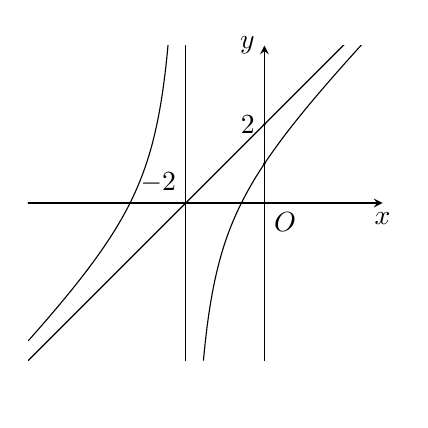
\begin{tikzpicture}[scale=0.5,>=stealth,line join=round,line cap=round]
		\draw[->]  (-6,0)--(3,0) node[below]{$x$};
		\draw[->] (0,-4)--(0,4) node[left]{$y$}; 
		\clip  (-6,-5) rectangle (3,4);
		\draw[samples=100,domain=-6:-2.2]  plot (\x,{(\x)+2-2/((\x)+2)});
		 \draw[samples=100,domain=-1.55:3] plot (\x,{(\x)+2-2/((\x)+2)});
		\draw[samples=100,domain=-6:3] plot (\x,{(\x)+2}); 
		 \draw[samples=100,domain=-4:4,smooth,variable=\y] plot ({-2},\y);
		\fill (-2,0) circle  (1pt) node[above left]{$-2$}
			(0,2) circle (1pt) node[left]{$2$} 
			(0,0) circle (1pt) node[below right]{$O$}; 
		\fill (0,0) circle (1pt); 
		\fill (0,1)  circle (1pt);
	\end{tikzpicture}
		 }
	\loigiai{ 
		\begin{itemchoice}
			\itemch {\bf  Đúng}.\\
			Vì $f(x)=\dfrac{x^2+4x+4-2}{x+2}=\dfrac{(x+2)^2-2}{x+2}=x+2-\dfrac{2}{x+2}$, $\forall x \ne -2$. 
			\itemch {\bf Sai}.\\ 
			$\lim\limits_{x\to 2^+}f(x)=\lim\limits_{x\to 2^+}\dfrac{x^2+4x+2}{x+2}=\dfrac{7}{2}\ne + \infty$ và $\lim\limits_{x\to 2^+}f(x)=\lim\limits_{x\to 2^+}\dfrac{x^2+4x+2}{x+2}=\dfrac{7}{2}\ne - \infty$ và $\lim\limits_{x\to 2^-}f(x)=\lim\limits_{x\to 2^-}\dfrac{x^2+4x+2}{x+2}=\dfrac{7}{2}\ne  +\infty$ và $\lim\limits_{x\to 2^-}f(x)=\lim\limits_{x\to 2^-}\dfrac{x^2+4x+2}{x+2}=\dfrac{7}{2}\ne -\infty$ nên đồ thị của hàm số không có đường tiệm cận đứng là $x=2$.
			\itemch {\bf Đúng}.\\ 
			Ta có $f(x)=x+2-\dfrac{2}{x+2}$ do  đó tiệm cận xiên của đồ thị hàm số đã cho là $y=x+2$.
			\itemch {\bf Đúng}.\\ 
			Vì đồ thị có tiệm cận đứng $x=-2$ và tiệm  cận xiên $y=x+2$.\\
			 Ta có $f'(x)=1+\dfrac{2}{(x+2)^2}>0$, $\forall x \ne -2$.\\
			Do đó, hàm  số đồng biến trên khoảng xác định. Thỏa mãn hình vẽ.
		\end{itemchoice}
	} 
\end{ex}

% nguồn: Phan1_Lop_12_Dai_so_Chuong_1
\begin{ex}%[2D1H4-1]%[ma:b9b0c73e]
	Cho hàm số $y=\dfrac{x^2-2x+3}{x-1}$ có đồ thị là  $(C)$.
	 \choiceTF
		{\True Đồ thị hàm số có hai đường  tiệm cận}
		{\True Đường tiệm cận xiên của đồ thị tạo với hai  trục tọa độ một tam giác vuông cân}
		{\True Giao điểm của  hai đường tiệm cận nằm trên trục hoành}
		{Đường tiệm cận xiên của đồ thị song song với đường  thẳng $x+y=0$}
	 \loigiai{
		\begin{itemchoice}
			 \itemch Đồ thị hàm số có hai đường tiệm cận: đường tiệm cận đứng có phương trình $x = 1$ và đường tiệm cận ngang có phương trình $y = x - 1$.
			\itemch Đường tiệm cận xiên của đồ thị hàm số cắt hai trục toạ độ $Ox$, $Oy$ lần lượt tại hai điểm $A(1; 0)$, $B(0; -1)$ nên tam giác $OAB$ là tam giác vuông  cân.
			\itemch Giao điểm hai  tiệm cận của đồ thị là $A(1; 0)$ nằm trên trục hoành.
			\itemch Đường tiệm cận xiên của đồ thị  $y = x - 1$ vuông góc với đường thẳng $y = -x$.
		\end{itemchoice}
	 }
\end{ex}

% nguồn: Phan1_Lop_12_Dai_so_Chuong_1
\begin{ex}%[2D1H4-1]%[ma:2ccec55b]
	\immini {Cho hàm số $y=\dfrac{x^2-x+1}{x-1}$ có đồ thị $(C)$  như hình vẽ.
	 \choiceTF
		{\True Đường thẳng $x=1$ là tiệm  cận đứng của đồ thị $(C)$}
		{$\lim\limits_{x \to  +\infty}\dfrac{f(x)}{x}=-1$}
		 {$\lim\limits_{x \to +\infty}\left[f(x)-x\right]=1$}
		{\True  Đường thẳng $y=x$ là tiệm cận xiên của đồ thị $(C)$}
		 }
		{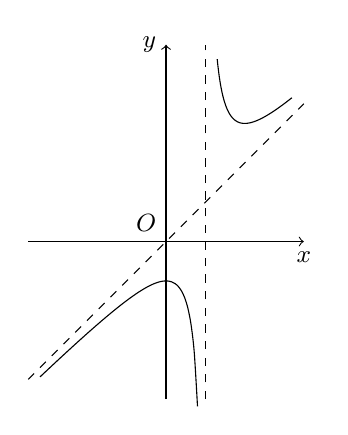
\begin{tikzpicture}[scale=0.5]
		\draw[->]  (-3.5,0) -- (3.5,0) node[below] {\small $x$};
		\draw[->] (0,-4) -- (0,5) node[left]  {\small $y$};
		\node at (0,0) [above left] {\small  $O$};
		\draw[dashed]  (1,-4) -- (1,5);
		\draw[dashed]  (-3.5,-3.5) -- (3.5,3.5);
		 \draw[domain=-3.2:0.8,smooth,samples=50]
			 plot (\x,{(\x*\x - \x + 1)/(\x - 1)});
		 \draw[domain=1.3:3.2,smooth,samples=200]
			plot (\x,{(\x*\x - \x + 1)/(\x - 1)}); 
	\end{tikzpicture}
		 }
	\loigiai{ 
		\begin{itemchoice}
			 \itemch Đường thẳng $x=1$ là tiệm cận đứng của đồ thị $(C)$.
			\itemch  $\lim\limits_{x \to +\infty}\dfrac{f(x)}{x}=\lim\limits_{x \to +\infty}\dfrac{x^2-x+1}{x^2-x}=1$.
			\itemch $\lim\limits_{x  \to +\infty}\left[f(x)-x\right]=\lim\limits_{x \to +\infty}\dfrac{1}{x-1}=0$.
			\itemch  Đường tiệm cận xiên của đồ thị $(C)$ là $y=x$.
		\end{itemchoice}
	} 
\end{ex}

% nguồn: Phan1_Lop_12_Dai_so_Chuong_1
\begin{ex}%[2D1H4-1]%[ma:1ec081c1]
	Cho  hàm số $y=\dfrac{5-4x}{2x+3}$ có đồ thị là $(C)$.
	\choiceTF 
		{\True Hàm số  đã cho không có cực trị}
		{Đồ thị hàm số  có tiệm cận đứng $x=-3$}
		{\True  Đồ thị hàm số có tiệm cận ngang $y=-2$}
		{\True Các đường tiệm cận của đồ thị hàm số tạo với  hai trục toạ độ một hình chữ nhật có diện tích bằng $3$}
	 \loigiai{
		Tập xác  định $\mathscr{D}=\mathbb{R} \backslash\left\{-\frac{3}{2}\right\}$.
		\begin{itemize}
			 \item $\lim\limits_{x \rightarrow-\left(\frac{3}{2}\right)^{+}} y=+\infty$; $\lim\limits_{x \rightarrow-\left(\frac{3}{2}\right)^-} y=-\infty$ nên đồ thị hàm số có tiệm cận đứng $x=-\dfrac{3}{2}$.
			\item $\lim\limits_{x \rightarrow-\infty} y=-2$; $\lim\limits_{x \rightarrow+\infty} y=-2$ nên đồ thị hàm số có  tiệm cận ngang $y=-2$.
		\end{itemize}
		Diện tích hình chữ nhật cần tìm  là $S=\left|-\dfrac{3}{2}\right| \cdot\left|2\right|=3$ (đvdt).
		\begin{itemchoice}
			\itemch  Hàm số đã cho không có cực trị.
			\itemch Đồ thị hàm số có  tiệm cận đứng $x=-\dfrac{3}{2}$.
			\itemch Đồ thị hàm  số có tiệm cận ngang $y=-2$.
			\itemch Các đường tiệm cận của đồ thị hàm số tạo với hai trục toạ độ một hình chữ nhật có diện tích bằng $3$. 
		\end{itemchoice}
	 }
\end{ex}

% nguồn: Phan1_Lop_12_Dai_so_Chuong_1
\begin{ex}%[2D1V4-1]%[ma:1b0baddf]
	Cho hàm số $y=\dfrac{x^2 + 2x - 1}{x - 1}$ và đồ thị của nó là~$(C)$. Xét tính đúng sai các khẳng  định sau.
	\choiceTF 
		{\True Hàm số có $2$ điểm cực trị} 
		{\True Đồ thị $(C)$ có tiệm cận đứng là~đường thẳng $x  = 1$}
		{Hàm số nghịch biến trên khoảng $(0;2)$} 
		{$M$ là~điểm bất kì thuộc đồ thị $(C)$. Tích khoảng cách từ $M$ đến  tiệm cận đứng và tiệm cận xiên của đồ thị $(C)$ bằng $\sqrt{2}$}
	\loigiai{ 
		\begin{itemchoice}
			\itemch 
			Ta có $y' = \dfrac{(2x+2)(x-1) -  (x^2+2x-1)}{(x-1)^2} = \dfrac{x^2 - 2x - 1}{(x-1)^2}$.
			\[ 
			 y' = 0 \Leftrightarrow x^2 - 2x - 1 = 0 \Leftrightarrow x = 1 \pm \sqrt{2}.
			 \]
			Vậy hàm số đã cho có 2 cực  trị.
			 \itemch Ta có
			 \[
			\lim_{x \to 1^+} \dfrac{x^2 +  2x - 1}{x-1} = +\infty.
			\] 
			Vậy $x  = 1$ là~tiệm cận đứng của đồ thị hàm số.
			\itemch Bảng  biến thiên
			\begin{center}
				
\begin{tikzpicture}
					 \tkzTabInit[nocadre,lgt=1.2,espcl=2.5,deltacl=0.6]{$x$/0.6,$y'$/0.6,$y$/2}
						 {$-\infty$,$1-\sqrt{2}$,$1$,$1-\sqrt{2}$,$+\infty$}
					\tkzTabLine  {,+,0,-,d,-,0,+,}
					\tkzTabVar{-/$-\infty$,+/$f (1-\sqrt{2})$,-D+/$-\infty$ /$+\infty$,-/$f  (1+\sqrt{2})$,+/$+\infty$}
				\end{tikzpicture}
			\end{center}
			Từ bảng biến thiên ta thấy hàm số nghịch biến trên $\left(1 - \sqrt{2};  1\right)$ và $\left(1; 1 + \sqrt{2}\right)$.
			\itemch Ta có tiệm cận xiên của đồ  thị hàm số là~$y = x + 3$ ($d_1$).\\
			 Tiệm cận đứng của đồ thị hàm số là~$x = 1$ ($d_2$).\\
			Với $M$ bất kì thuộc đồ thị hàm số, $M\left(a; \dfrac{a^2  + 2a - 1}{a - 1}\right)$.\\
			Ta  có
			\[ 
			\mathrm{d}(M, d_1) = \dfrac{\left| a +  3 - \dfrac{a^2 + 2a - 1}{a - 1} \right|}{\sqrt{2}} = \dfrac{|-2|}{\sqrt{2}} = \sqrt{2}.
			\] 
			 \[
			 \mathrm{d}(M, d_2) = |a - 1|.
			 \]
			Tích khoảng cách từ  $M$ đến tiệm cận đứng và tiệm cận xiên của đồ thị (C) bằng $\sqrt{2} \cdot |a - 1|$.
	\end{itemchoice}}
\end{ex}

% nguồn: Phan1_Lop_12_Dai_so_Chuong_1
\begin{ex}%[2D1V4-1]%[ma:fae6d414]
	Cho hàm số $y=f(x)$ xác định trên  $\mathbb{R}\setminus\{1\}$, liên tục trên mỗi khoảng xác định và có bảng biến thiên như sau
	\begin{center}
		
\begin{tikzpicture}[scale=1,font=\footnotesize,line join=round,line cap=round,>=stealth]
			 \tkzTabInit[espcl=3,lgt=1.5]
				{$x$/0.7,$y'$/0.7,$y$/2.1} 
				{$-\infty$,$1$,$2$,$+\infty$} 
			\tkzTabLine{,-,d,-,0,+,} 
			\tkzTabVar{+/$3$,-D+/$-\infty$/$+\infty$,-/$-2$,+/$5$} 
		\end{tikzpicture}
	\end{center}
	 \choiceTF
		{Hàm số  đã cho nghịch biến trên khoảng $(-\infty;2)$ và đồng biến trên khoảng $(2;+\infty)$}
		{\True Đồ thị hàm số $y=f(x)$ có một đường tiệm cận đứng  là $x=1$}
		{\True Đồ thị hàm số $y=f(x)$ có một đường tiệm cận ngang là  $y=3$}
		{\True Đồ  thị hàm số $y=\dfrac{1}{f(x)+2}$ có hai đường tiệm cận đứng}
	\loigiai{ 
		\begin{itemchoice}
			\itemch Hàm số  đã cho nghịch biến trên mỗi khoảng $(-\infty;1)$; $(1;2)$ và đồng biến trên khoảng $(2;+\infty)$.
			 \itemch Do $\lim\limits_{x \rightarrow 1^{-}} y=-\infty$ nên đồ thị hàm số có một đường tiệm cận đứng là $x=1$.
			\itemch Do $\lim\limits_{x \rightarrow-\infty} y=3$ nên đồ thị hàm số  có một đường tiệm cận ngang là $y=3$.
			\itemch Dựa vào đồ thị, ta có $f(x)+2=0 \Leftrightarrow f(x)=-2 \Leftrightarrow\hoac{&x=2\\&x=x_0\in (-\infty;1).}$\\ 
			Hàm  số $y=g(x)=\dfrac{1}{f(x)+2}$ có tập xác định $\mathscr{D}=\mathbb{R}\setminus\left\{x_{0};1;2\right\}$.\\
			Hàm số $y=g(x)$ liên tục trên mỗi khoảng xác định của  nó.\\
			Các giới hạn $\lim\limits_{x \rightarrow x_0^+} \dfrac{1}{f(x)+2}=-\infty$; $\lim\limits_{x \rightarrow 1^-} \dfrac{1}{f(x)+2}=0$; $\lim\limits_{x\rightarrow 1^+} \dfrac{1}{f(x)+2}=0$; $\lim\limits_{x \rightarrow 2^-} \dfrac{1}{f(x)+2}=+\infty$.\\ 
			Vậy hàm số $y=g(x)=\dfrac{1}{f(x)+2}$ có hai đường tiệm cận  đứng là $x=x_0$ và $x=2$.
		\end{itemchoice}
	} 
\end{ex}


%%%%%%%%%%%%%%%% TRẢ LỜI NGẮN %%%%%%%%%%%%%%%%

% nguồn: Phan2_Lop_12_Dai_so_Chuong_1
\begin{bt}%[2D1N4-1]%[ma:53eb578e]
	 Cho hàm số $y = \dfrac{2x-1}{x+3}$. Gọi $x=m$ và $y=n$ lần lượt là đường tiệm cận đứng và tiệm cận ngang của đồ thị hàm số. Tính giá trị của biểu thức $P=\dfrac{2m-1}{n+3}$.
	 \shortans{-1,4}
	\loigiai{Ta  có
		\begin{itemize}
			\item $\lim\limits_{x \to  -3} y = \infty \Rightarrow$ đường thẳng $x=-3$ là đường tiệm cận đứng.
			\item $\lim\limits_{x \to +\infty} y = 2$  và $\lim\limits_{x \to -\infty} y = 2 \Rightarrow$ đường thẳng $ y = 2$ là đường tiệm cận ngang.
		\end{itemize}
		Vậy $m=-3$; $n=2 \Rightarrow P = \dfrac{2\cdot(-3)-1}{2+3} =  \dfrac{-7}{5} = -1{,}4$.
	} 
\end{bt}

% nguồn: Phan2_Lop_12_Dai_so_Chuong_1
\begin{bt}%[2D1N4-1]%[ma:2cc26468]
	Cho hàm  số $y = \dfrac{-x - 3}{4x + 1}$. Tọa độ tâm đối xứng của đồ thị hàm số có dạng $A(m; n)$. Tính $m + n$.
	 \shortans{-0,5}
	 \loigiai{Ta có
		\begin{itemize}
			 \item $\lim\limits_{x \to +\infty} y = -\dfrac{1}{4}$; $\lim\limits_{x \to +\infty} y = -\dfrac{1}{4} \Rightarrow$ đường thẳng $y = -\dfrac{1}{4}$ là đường tiệm cận ngang.
			\item  $\lim\limits_{x \to -\frac{1}{4}^+} y = -\infty$; $\lim\limits_{x \to -\frac{1}{4}^-} y= +\infty \Rightarrow =$ đường thẳng $x = -\dfrac{1}{4}$ là đường tiệm cận đứng.
		\end{itemize}
		Vậy $m + n =  -0{,}5$.
	} 
\end{bt}

% nguồn: Phan2_Lop_12_Dai_so_Chuong_1
\begin{bt}%[2D1N4-1]%[ma:01980fc7]
	Cho các hằng số $a$, $b$, $c$, $d$ khác $0$ thoả mãn $a d-b c \neq 0$. Tổng số đường tiệm cận ngang và đường tiệm cận đứng của đồ thị hàm số $y=\dfrac{a x+b}{c x+d}$ là  bao nhiêu?
	\shortans{2} 
	 \loigiai{
		Đường tiệm  cận đứng của đồ thị hàm số là $x=-\dfrac{d}{c}$.\\
		Đường tiệm cận ngang của đồ thị hàm số là $y=\dfrac{a}{c}$.\\ 
		 Vậy có $2$ đường tiệm cận.
	 }
\end{bt}

% nguồn: Phan2_Lop_12_Dai_so_Chuong_1
\begin{bt}%[2D1H4-1]%[ma:d3b92baf]
	Cho hàm số $y = \dfrac{x^3 - 9x}{x^3 - x^2 -  5x - 3}$ có đồ thị là $(C)$. Tổng số đường tiệm cận đứng và tiệm cận ngang của đồ thị $(C)$ là bao nhiêu?
	\shortans{2} 
	\loigiai{ 
		Tập xác định: $\mathscr{D} =  \mathbb{R} \setminus \{-1; 3\}$ và có $\lim\limits_{x \to \pm\infty} y = 1$ nên đường thẳng $y = 1$ là tiệm cận ngang.
		\begin{itemize}
			\item $\lim\limits_{x \to -1} y = \lim\limits_{x \to -1} \dfrac{x(x - 3)(x +  3)}{(x - 3)(x + 1)^2} = -\infty$ nên đường thẳng $x = -1$ là tiệm cận đứng.
			\item $\lim\limits_{x \to 3} y = \lim\limits_{x \to 3} \dfrac{x(x - 3)(x + 3)}{(x  - 3)(x + 1)^2} = \lim\limits_{x \to 3} \dfrac{x(x + 3)}{(x + 1)^2} = \dfrac{18}{16} = \dfrac{9}{8}$ nên đường thẳng $x = 3$ không là tiệm cận đứng.
		\end{itemize}
		Tổng số đường tiệm cận đứng và tiệm cận ngang của đồ  thị $(C)$ là $2$.
	 }
\end{bt}

% nguồn: Phan2_Lop_12_Dai_so_Chuong_1
\begin{bt}%[2D1H4-1]%[ma:fe7a658a]
	Cho đồ thị hàm số $f(x)=5 x-1+\dfrac{8}{x-1}$ có tâm đối xứng là $I(a;b)$. Giá trị của biểu thức $C=a+3 b$ là  bao nhiêu?
	\shortans{-19} 
	\loigiai{ 
		Ta có $a=\lim\limits_{x\to +\infty}\dfrac{f(x)}{x}=\lim\limits_{x\to +\infty} \left(5-\dfrac{1}{x}+\dfrac{8}{x(x-1)}\right)=5$.\\ 
		Ta có $b=\lim\limits_{x\to +\infty} \big[f(x)-5x\big]=\lim\limits_{x\to +\infty} \left(5x-1+\dfrac{8}{x-1}-5x\right)=-1$.\\ 
		Do đó, đồ  thị hàm số có tiệm cận xiên là $y=5x-1$.\\
		 Mặt khác, $x=-1$ là tiệm cận đứng của đồ thị hàm số.\\
		Ta có tâm đối xứng của đồ thị hàm số trên là  giao điểm của $y=5x-1$ và $x=-1$.\\
		Vậy  $I(-1;-6)$.\\
		Suy ra $C=a+3b=-19$. 
	 }
\end{bt}

% nguồn: Phan2_Lop_12_Dai_so_Chuong_1
\begin{bt}%[2D1H4-1]%[ma:c76aaafc]
	Cho đồ thị hàm số $y=\dfrac{3x+2}{x-4}$ có đường  tiệm cận đứng $x=a$ và đường tiệm cận ngang $y=b$ với $a$, $b\in \mathbb{R}$. Giá trị của biểu thức $C=5a+6b$ là bao nhiêu?
	\shortans{38} 
	 \loigiai{
		Đồ thị hàm số có  tiệm cận đứng $x=4$ và tiệm cận ngang $y=3$.\\
		Suy  ra $\heva{&a=4\\&b=3}$ nên $C=5a+6b=5 \cdot 4+6 \cdot 3=38$.
	} 
\end{bt}

% nguồn: Phan2_Lop_12_Dai_so_Chuong_1
\begin{bt}%[2D1H4-1]%[ma:32ac1c1b]
	Gọi $I(a; b)$ là giao điểm của đường tiệm cận đứng và đường tiệm cận ngang của đồ thị  hàm số $y = \dfrac{x - 2}{x + 2}$. Tính $T = a + b$.
	\shortans{-1} 
	\loigiai{ 
		Hàm số $y = \dfrac{x - 2}{x + 2}$ có tập xác định $\mathscr{D} = \mathbb{R} \setminus \{-2\}$. 
		\begin{itemize}
			\item $\lim\limits_{x \to -\infty} y = 1$ và $\lim\limits_{x \to -\infty} y = 1$ nên đồ thị hàm số có đường tiệm cận ngang  là đường thẳng $y = 1$.
			\item $\heva{&\lim\limits_{x \to (-2)^-} y = +\infty\\&\lim\limits_{x \to (-2)^+} y = -\infty}$ nên đồ thị hàm số có đường tiệm cận đứng  là đường thẳng $x = -2$.
		\end{itemize}
		Vậy giao điểm của đường tiệm cận đứng và đường tiệm cận ngang của đồ thị hàm số đã  cho là điểm $I(-2; 1)$ nên $T = -2 + 1 = -1$.
	} 
\end{bt}

% nguồn: Phan2_Lop_12_Dai_so_Chuong_1
\begin{bt}%[2D1H4-1]%[ma:b1248c9b]
	Tính tổng số đường tiện cận đứng và tiệm cận ngang của đồ thị  hàm số $y=\dfrac{x^2+2x+3}{x^2-4}$.
	\shortans{3} 
	 \loigiai{
		Tập xác định  $\mathscr{D}=\mathbb{R}\setminus \{-2;2\}$.\\
		Ta có $\lim\limits_{x  \to (-2)^+}y=+\infty$; $\lim\limits_{x \to (-2)^-}y=-\infty \Rightarrow x=-2$ là tiệm cận đứng của đồ thị hàm số.\\
		Tương tự đồ thị hàm số có  thêm một tiệm cận đứng khác là $x=2$.\\
		Ta có $\lim\limits_{x \to -\infty} f(x) = 1; \quad \lim\limits_{x \to +\infty} f(x) = 1 \Rightarrow y = 1$ là tiệm  cận ngang của đồ thị hàm số.\\
		Vậy tổng số đường tiệm cận đứng và tiệm cận ngang của đồ thị hàm số  là $3$.
	 }
\end{bt}

% nguồn: Phan2_Lop_12_Dai_so_Chuong_1
\begin{bt}%[2D1H4-1]%[ma:c2a1eeeb]
	Cho hàm số $y=\dfrac{x^2}{x-3}$ có đường tiệm cận xiên $y=ax+b$ với $a, b \in \mathbb{R}$. Giá  trị của biểu thức $D=a-b^2$ là bao nhiêu?
	\shortans{-8} 
	 \loigiai{
		Ta có  $y=\dfrac{x^2}{x-3}=x+3+\dfrac{9}{x-3}$.\\
		Do $\lim\limits_{x \to +\infty} [y-(x+3)]=\lim\limits_{x \to +\infty} \dfrac{9}{x-3}  =0$ nên đồ thị hàm số có tiệm cận xiên là đường thẳng có phương trình $y=x+3$.\\
		Suy ra $\heva{&a=1\\&b=3}$ nên $D=a-b^2=1-3^2=-8$. 
	} 
\end{bt}

% nguồn: Phan2_Lop_12_Dai_so_Chuong_1
\begin{bt}%[2D1H4-1]%[ma:48e2138c]
	Biết rằng đồ thị hàm số $y=\dfrac{ax+1}{bx-2}$  có tiệm cận đứng là $x=2$ và tiệm cận ngang là $y=3$. Tính giá trị biểu thức $a-2b$.
	\shortans{1} 
	\loigiai{Tiệm cận đứng của đồ thị hàm  số $y=\dfrac{ax+1}{bx-2}$ là $x=\dfrac{2}{b}$.\\
		Tiệm cận ngang của đồ thị  hàm số $y=\dfrac{ax+1}{bx-2}$ là $y=\dfrac{a}{b}$.\\
		Theo  giả thiết ta có: $\heva{&\dfrac{2}{b}=2\\&\dfrac{a}{b}=3}\Rightarrow \heva{&a=3\\&b=1}\Rightarrow a-2b=3-2\cdot 1=1$.
	} 
\end{bt}

% nguồn: Phan2_Lop_12_Dai_so_Chuong_1
\begin{bt}%[2D1H4-1]%[ma:1a227111]
	Cho đồ thị hàm số $f(x)=\dfrac{3 x+5}{-x+7}$ có tâm đối xứng  là $I(a; b)$. Giá trị của biểu thức $B=-4 a-b$ là bao nhiêu?
	 \shortans{-25}
	 \loigiai{
		Ta có tiệm cận đứng của đồ thị hàm số là $x=7$, tiệm cận ngang  của đồ thị hàm số là $y=-3$.\\
		Suy  ra $I(7;-3)$.\\
		Vậy $B=-4a-b=-25$. 
	 }
\end{bt}

% nguồn: Phan2_Lop_12_Dai_so_Chuong_1
\begin{bt}%[2D1H4-1]%[ma:467fb564]
	Cho đồ thị hàm số $y = x - \sqrt{x^2+x-4}$ có một đường tiệm cận ngang là đường thẳng $y = \dfrac{m}{n}$. Khi  đó $\dfrac{m}{n}$ bằng
	\shortans{-0,5} 
	\loigiai{Ta  xét $\lim\limits_{x \to +\infty} y = -\dfrac{1}{2}$; $\lim\limits_{x \to -\infty} y = -\infty \Rightarrow y = -\dfrac{1}{2}$ là đường tiệm cận ngang.
	} 
\end{bt}

% nguồn: Phan2_Lop_12_Dai_so_Chuong_1
\begin{bt}%[2D1H4-1]%[ma:5a9405f7]
	Tìm hệ  số góc $k$ của đường tiệm cận xiên của đồ thị hàm số $y = \dfrac{2x^3 + 5x^2 - 1}{x^2 - x + 1}$.
	 \shortans{2}
	\loigiai{ 
		Tập xác định $\mathscr{D}  = \mathbb{R}$ nên hàm không có tiệm cận đứng.\\
		Ta có 
		$a = \lim\limits_{x \to \pm\infty} \dfrac{f(x)}{x} = \lim\limits_{x \to \pm\infty} \dfrac{2x^3 + 5x^2 - 1}{x\left(x^2 - x + 1\right)} = \lim\limits_{x \to \pm\infty} \dfrac{2  + \dfrac{5}{x} - \dfrac{1}{x^3}}{1 - \dfrac{1}{x} + \dfrac{1}{x^2}} = 2$.\\
		 $
		b =  \lim\limits_{x \to \pm\infty} \left( y - 2x \right) = \lim\limits_{x \to \pm\infty} \left( \dfrac{2x^3 + 5x^2 - 1}{x^2 - x + 1} - 2x \right) = \lim\limits_{x \to \pm\infty} \dfrac{7x^2 - 2x - 1}{x^2 - x + 1} = 7$.\\
		$\Rightarrow y = 2x + 7$ là tiệm cận xiên của đồ thị hàm số và có hệ số góc $k =  2$.
	 }
\end{bt}

% nguồn: Phan2_Lop_12_Dai_so_Chuong_1
\begin{bt}%[2D1V4-1]%[ma:81f9e9b0]
	Diện tích hình chữ nhật tạo bởi hai đường tiệm cận của đồ thị hàm số $y = \dfrac{2x  + 1}{x + 3}$ và các trục tọa độ bằng bao nhiêu?
	\shortans{6} 
	\loigiai{ 
		Đường tiệm cận đứng của đồ thị  hàm số $x = -3$;\\
		Đường tiệm cận ngang của đồ thị hàm số  $y = 2$.\\
		Hai đường tiệm cận tạo với các trục tọa độ một hình chữ nhật có chiều dài bằng $3$, chiều rộng  bằng $2$.\\
		Diện tích hình chữ  nhật $S = 2 \cdot 3 = 6$.
	} 
\end{bt}

% nguồn: Phan2_Lop_12_Dai_so_Chuong_1
\begin{bt}%[2D1V4-1]%[ma:403becf8]
	Cho đồ thị hai hàm số $f(x) = \dfrac{x + 1}{x - 1}$ và $g(x) = \dfrac{ax + 1}{x - 2}$, $a \ne -\dfrac{1}{2}$. Tìm giá trị thực dương của $a$ để các tiệm cận của hai đồ thị hàm số tạo thành một hình chữ nhật có  diện tích là $4$.
	\shortans{5} 
	\loigiai{ 
		Đồ thị hàm số $f(x)=\dfrac{x+1}{x-1}$ có hai đường tiệm  cận là $x=1$ và $y=1$.\\
		Đồ thị hàm số $g(x)=\dfrac{ax+1}{x-2}$ có hai đường tiệm  cận là $x=2$ và $y=a$.\\
		Hình chữ nhật được tạo thành từ bốn đường tiệm cận của hai đồ thị trên có hai kích thước  lần lượt là $1$ và $\left|a-1\right|$.\\
		Theo giả thiết, ta có $\left|a-1\right|\cdot 1=4 \Leftrightarrow \hoac{&a=5\\&a=-3}.$ Vì $a>0$ nên  chọn $a=5$.
	} 
\end{bt}

% nguồn: Phan2_Lop_12_Dai_so_Chuong_1
\begin{bt}%[2D1V4-1]%[ma:42619930]
	Cho hàm số $y=\dfrac{2x-1}{x+1}$ có đồ thị $(C)$. Tích các khoảng cách từ điểm $M$ bất kỳ thuộc $(C)$  đến hai đường tiệm cận bằng bao nhiêu?
	 \shortans{3}
	 \loigiai{
		Đồ thị $(C)$ có đường  tiệm cận đứng là $\Delta_1\colon x=-1\Leftrightarrow x+1=0$.\\
		Đường tiệm cận ngang là $\Delta_2 \colon y=2  \Leftrightarrow y-2=0$.\\
		Giả sử $M\left(x_0;\dfrac{2x_0-1}{x_0+1}\right)\in (C)$, $x_0\neq -1$.\\ 
		 Ta có $\mathrm{d}\left(M;\Delta_1\right)=\left|x_0+1\right|$ và $\mathrm{d}\left(M;\Delta_2\right)=\left|\dfrac{2x_0-1}{x_0+1}-2\right|=\dfrac{3}{\left|x_0+1\right|}$.\\
		Suy ra $\mathrm{d}\left(M;\Delta_1\right)\cdot  \mathrm{d}\left(M;\Delta_2\right)=\left|x_0+1\right| \cdot \dfrac{3}{\left|x_0+1\right|}=3$.
	} 
\end{bt}

% nguồn: Phan2_Lop_12_Dai_so_Chuong_1
\begin{bt}%[2D1V4-1]%[ma:224eda4d]
	 Cho hàm số $y = \dfrac{ax^2 + x - 1}{4x^2 + bx + 9}$ có đồ thị $(C)$ và $a$, $b$ là các hằng số dương thỏa mãn $a\cdot b = 4$. Biết rằng $(C)$ có đường tiệm cận ngang $y = c$ và có đúng $1$ đường tiệm cận đứng. Tính tổng $T = 3a + b - 24c$.
	 \shortans{11}
	 \loigiai{
		Theo giả  thiết $a > 0$, $b > 0$.\\
		Với $ab = 4$ ta có 
		$ 
		y = \dfrac{ax^2 + x - 1}{4x^2 + bx + 9} = \dfrac{\dfrac{4}{b}x^2 + x - 1}{4x^2 + bx + 9} = \dfrac{4x^2 + bx - b}{b(4x^2 + bx +  9)} = \dfrac{1}{b} -\dfrac{b+9}{b\left(4x^2+bx+9\right)}.
		$\\ 
		Đồ thị $(C)$ có đúng $1$ đường tiệm cận  đứng nên $4x^2 + bx + 9 = 0$ có nghiệm kép\\
		Suy ra $\Delta = b^2 - 4 \cdot 4 \cdot 9 =  0 \Leftrightarrow b = 12$ (do $b > 0$).\\
		Ta có $ab = 4$ suy ra $a = \dfrac{1}{3}$; $c =  \lim\limits_{x \to +\infty} \dfrac{ax^2 + x - 1}{4x^2 + bx + 9}
		= \lim\limits_{x \to +\infty} \dfrac{a + \dfrac{1}{x} - \dfrac{1}{x^2}}{4 +  \dfrac{b}{x} + \dfrac{9}{x^2}}
		=  \dfrac{a}{4} \Rightarrow c = \dfrac{1}{12}$.\\
		Vậy $T = 3a + b - 24c  = 11$.
	 }
\end{bt}

% nguồn: Phan2_Lop_12_Dai_so_Chuong_1
\begin{bt}%[2D1V4-1]%[ma:eff7c6e5]
	Cho hàm số $\dfrac{2x+2}{2x-3}$ có đồ thị $(C)$. Có bao nhiêu điểm $M$ thuộc $(C)$ sao cho khoảng cách từ điểm $M$ đến đường tiệm cận ngang bằng $10$ lần khoảng cách từ điểm $M$ đến đường tiệm cận  đứng.
	\shortans{2} 
	 \loigiai{
		Ta có các đường thẳng $x=\dfrac{3}{2}$ và $y=1$ lần lượt là đường tiệm cận đứng và đường tiệm cận ngang  của đồ thị hàm số mà $M\in (C)\Rightarrow M\left(x;\dfrac{2x+2}{2x-3}\right)$ với $x\neq \dfrac{3}{2}$.\\
		Khoảng  cách từ điểm $M$ đến đường tiệm cận đứng bằng $\left|x-\dfrac{3}{2}\right|=\dfrac{\left|2x-3\right|}{2}$.\\
		Khoảng cách từ điểm $M$ đến đường tiệm cận ngang bằng  $\left|\dfrac{2x+2}{2x-3}-1\right|=\dfrac{5}{\left|2x-3\right|}$.\\
		Khi đó: $\dfrac{5}{\left|2x-3\right|}=10\cdot \dfrac{\left|2x-2\right|}{2}\Leftrightarrow \left(2x-3\right)^2=1\Leftrightarrow 4x^2-12x+8=0\Leftrightarrow \hoac{&x=2\\&x=1}\Rightarrow \hoac{&M(2;6)\\&M(1;-4).}$\\ 
		Vậy có $2$ điểm $M$  thỏa mãn yêu cầu bài toán.
	 }
\end{bt}

% nguồn: Phan2_Lop_12_Dai_so_Chuong_1
\begin{bt}%[2D1V4-1]%[ma:fef7bf1a]
	Cho hàm số $y=\dfrac{2x-1}{x-1}$ có đồ thị $(C)$. Gọi $M(a;b)$ là điểm thuộc đồ thị hàm số có hoành độ dương sao cho tổng khoảng cách từ $M$  đến hai tiệm cận của $(C)$ nhỏ nhất. Khi đó tổng $a+2b$ bằng bao nhiêu?
	\shortans{8} 
	 \loigiai{
		Hàm số $y = \dfrac{2x - 1}{x - 1}$ có đường tiệm cận ngang $ y = 2 $ và đường tiệm cận đứng \( x  = 1 \). Khi đó\\
		Khoảng cách từ $ M(a; b)$ đến tiệm cận ngang là $\left|b-2\right|=\left|\dfrac{2a-1}{a-1}-2\right|=\dfrac{1}{\left|a-1\right|}$ do $\big(M\in (C)\big)$.\\ 
		Khoảng cách từ $M(a; b)$ đến tiệm cận đứng là $\left|a  - 1\right|$.\\
		Ta có  $\left|a-1\right|+\dfrac{1}{\left|a-1\right|}\geq 2\sqrt{\left|a-1\right|\cdot \dfrac{1}{\left|a-1\right|}}=2$.\\
		 Vậy tổng khoảng cách nhỏ nhất là $2$ khi
		\begin{eqnarray*}
			&&\left|a  - 1\right| = \dfrac{1}{\left|a-1\right|}\\
			 &\Leftrightarrow& \left(a-1\right)^2=1\\
			 &\Leftrightarrow& a^2-2a=0\\
			&\Leftrightarrow& \hoac{&a= 0~ \text{ (loại)}\\&a=2.} 
		\end{eqnarray*}
		 $\Rightarrow b=\dfrac{2\cdot2-1}{2-1}=3 \Rightarrow a+2b=8$.
	 }
\end{bt}


%%%%%%%%%%%%%%%% TỰ LUẬN %%%%%%%%%%%%%%%%

% nguồn: Phan2_Lop_12_Dai_so_Chuong_1
\begin{bt}%[2D1N4-1]%[ma:9e1e9ba4]
	Xác định tiệm cận xiên của đồ thị hàm số cho bởi  công thức sau:
	\begin{listEX}[2]
		\item  $y=f(x)=x+\dfrac{1}{x+2}$.
		\item $y=f(x)=\dfrac{x^2-x+2}{x+1}$. 
	\end{listEX}
	\loigiai{ 
		\begin{listEX}
			 \item
			 Ta có$\lim\limits_{x \to +\infty} \left[f(x)-x\right]=\lim\limits_{x \to +\infty}\dfrac{1}{x+2}=0$. Tương tự $\lim\limits_{x \to -\infty}\left[f(x)-x\right]=0$.\\
			Vậy đồ thị hàm số $f(x)$ có tiệm  cận xiên là đường thẳng $y=x$.
			 \item
			Ta có: $a=\lim\limits_{x \to +\infty}\dfrac{f(x)}{x}=\lim\limits_{x \to +\infty}\dfrac{x^2-x+2}{x^2+x}=1$; $b=\lim\limits_{x \to -\infty}\left[f(x)-x\right]=\lim\limits_{x  \to -\infty}\dfrac{-2x+2 }{x+1}=-2$.\\
			 Tương tự $\lim\limits_{x \to -\infty}\dfrac{f(x)}{x}=1$, $\lim\limits_{x \to -\infty}\left[f(x)-x\right]=-2$.\\
			Vậy đồ thị hàm số $f(x)$  có tiệm cận xiên là đường thẳng $y=x-2$.
		\end{listEX}
	 }
\end{bt}

% nguồn: Phan2_Lop_12_Dai_so_Chuong_1
\begin{bt}%[2D1N4-1]%[ma:cd6677b1]
	Xác định tiệm cận đứng của đồ  thị hàm số cho bởi công thức sau
	\begin{listEX}[2]
		\item $y=f(x)=\dfrac{3-x}{x+2}$. 
		\item  $y=f(x)=\dfrac{x^{2}+2}{x}$.
	\end{listEX}
	 \loigiai{
		\begin{enumerate}
			\item Ta có $\lim\limits_{x \rightarrow 2^{+}}  f(x)=\lim\limits_{x \rightarrow 2^{+}} \dfrac{3-x}{x+2}=+\infty$. \\Tương tự, $\lim\limits_{x \rightarrow-2^{-}} f(x)=-\infty$.\\
			Vậy đồ thị hàm số $f(x)$ có tiệm cận đứng là đường thẳng $x=-2$. 
			\item Ta có: $\lim\limits_{x \rightarrow 0^{+}} f(x)=\lim\limits_{x \rightarrow 0^{+}} \dfrac{x^{2}+2}{x}=+\infty$. \\Tương tự, $\lim\limits_{x \rightarrow 0^{-}} f(x)=-\infty$.\\ 
			Vậy đồ thị hàm số $f(x)$ có tiệm cận đứng là đường  thẳng $x=0$.
	\end{enumerate}}
\end{bt}

% nguồn: Phan2_Lop_12_Dai_so_Chuong_1
\begin{bt}%[2D1H4-1]%[ma:f89ce8db]
	Xác định tiệm cận đứng và tiệm cận ngang của đồ thị hàm số  cho bởi công thức sau
	\begin{listEX}[2]
		 \item $y=\dfrac{2x-1}{x+1}$.
		\item  $y=\dfrac{2x-3}{1-2x}$.
		 \item $y=\dfrac{x^2-5 x+4}{x^2-1}$.
		\item  $y=\dfrac{2x-1}{x^2-3x+2}$.
	\end{listEX}
	\loigiai{ 
		\begin{enumerate}
			\item Xét $\lim\limits_{x \rightarrow(-1)^+}\dfrac{2 x-1}{x+1}=-\infty$ (hoặc $\lim\limits_{x \rightarrow-1^-} \dfrac{2x-1}{x+1}=-\infty$) nên  đường thẳng $x=-1$ là tiệm cận đứng.\\
			 Xét $\lim\limits_{x\rightarrow \pm \infty} \dfrac{2x-1}{x+1}=2$ nên đường thẳng $y=2$ là tiệm cận ngang.
			\item Ta có $\lim\limits_{x \rightarrow \pm \infty}  \dfrac{2x-3}{1-2x}=-1$ suy ra $y=-1$ là tiệm cận ngang.\\
			Xét $\heva{&\lim\limits_{x \rightarrow \left(\frac{1}{2}\right)^+}\dfrac{2x-3}{1-2x}=+\infty\\&\lim\limits_{x \rightarrow  \left(\frac{1}{2}\right)^-}\dfrac{2x-3}{1-2x}=-\infty}$, suy ra $x=\dfrac{1}{2}$ là tiệm cận đứng.
			\item  Điều kiện xác định $x \neq \pm 1$\\
			 Ta có $\heva{&\lim\limits_{x \rightarrow \pm \infty}\dfrac{x^2-5x+4}{x^2-1}=1\\&\lim\limits_{x \rightarrow (-1)^-}\dfrac{x^2-5x+4}{x^2-1}=+\infty\\&\lim\limits_{x \rightarrow 1}\dfrac{x^2-5x+4}{x^2-1}=-\dfrac{3}{2}}$.\\
			Suy ra  hàm số có tiệm cận ngang là $y=1$ và một tiệm cận đứng là $x=-1$.
			\item Tập xác định $\mathscr{D}=\mathbb{R}  \setminus\{1;2\}$.
			\begin{itemize}
				\item $\lim\limits_{x \rightarrow \pm \infty} y=\lim\limits_{x \rightarrow \pm \infty} \dfrac{2 x-1}{x^2-3x+2}=0$, suy ra  $y=0$ là tiệm cận ngang.
				\item  $\lim\limits_{x\rightarrow 1^{-}} y=\lim _{x \rightarrow 1^-} \dfrac{2x-1}{x^2-3x+2}=\lim\limits_{x\rightarrow 1^-} \dfrac{2x-1}{(x-1)(x-2)}=+\infty$ và $\lim\limits _{x\rightarrow 1^+} y=-\infty$.\\
				Suy ra $x=1$ là đường tiệm cận  đứng.
				\item $\lim\limits_{x \rightarrow  2^{-}} y=\lim\limits_{x \rightarrow 2^{-}} \dfrac{2 x-1}{x^{2}-3 x+2}=\lim\limits_{x \rightarrow 1^{-}} \dfrac{2x-1}{(x-1)(x-2)}=-\infty$ và $\lim\limits _{x\rightarrow 2^+} y=+\infty$.\\
				Suy ra $x=2$ là đường  tiệm cận đứng.
			\end{itemize}
		\end{enumerate}
	} 
\end{bt}

% nguồn: Phan2_Lop_12_Dai_so_Chuong_1
\begin{bt}%[2D1H4-1]%[ma:82e2daed]
	 Xác định tiệm cận ngang của đồ thị hàm số cho bởi công thức sau
	\begin{listEX}[2]
		 \item $y=f(x)=\dfrac{3x-2}{x+1}$.
		\item  $y=f(x)=\dfrac{\sqrt{x^2+1}}{x}$.
	\end{listEX}
	\loigiai{ 
		\begin{enumerate}
			\item Ta có $\lim\limits_{x \rightarrow+\infty}  f(x)=\lim\limits_{x\rightarrow+\infty}\dfrac{3 x-2}{x+1}=\lim\limits_{x\rightarrow+\infty} \dfrac{3-\dfrac{2}{x}}{1+\dfrac{1}{x}}=3$. \\
			Tương  tự, $\lim\limits_{x\rightarrow-\infty} f(x)=3$.\\
			 Vậy đồ thị hàm số $f(x)$ có tiệm cận ngang là đường thẳng $y=3$.
			\item  Ta có
			\begin{itemize}
				\item  $\lim\limits_{x\rightarrow+\infty}f(x)=\lim\limits_{x\rightarrow+\infty} \dfrac{\sqrt{x^{2}+1}}{x}=\lim\limits_{x \rightarrow+\infty} \sqrt{\dfrac{x^{2}+1}{x^{2}}}=\lim\limits_{x \rightarrow+\infty}\sqrt{1+\dfrac{1}{x^{2}}}=1$.
				\item $\lim\limits_{x\rightarrow-\infty} f(x)=\lim\limits_{x \rightarrow-\infty} \dfrac{\sqrt{x^{2}+1}}{x}=\lim\limits_{x \rightarrow-\infty}\left(-\sqrt{\dfrac{x^{2}+1}{x^{2}}}\right)=\lim\limits_{x  \rightarrow-\infty}\left(-\sqrt{1+\dfrac{1}{x^{2}}}\right)=-1$.
			\end{itemize}
			 Vậy đồ thị hàm số $f(x)$ có hai tiệm cận ngang là $y=1$ và $y=-1$.
	\end{enumerate}}
\end{bt}

% nguồn: Phan2_Lop_12_Dai_so_Chuong_1
\begin{bt}%[2D1H4-1]%[ma:d334860e]
	Xác định tiệm cận đứng và tiệm cần xiên của đồ thị hàm số cho bởi công thức sau: 
	\begin{multicols}{3}
		\begin{enumerate}
			 \item $y=\dfrac{x^2+2}{2x-4}$
			\item $y=\dfrac{2x^2-3x-6}{x+2}$ 
			\item  $y=\dfrac{2x^2+9x+11}{2x+5}$
		\end{enumerate}
	\end{multicols}
	\loigiai{ 
		\begin{listEX}
			\item Hàm số có tập xác định $\mathscr{D}=\mathbb{R}\setminus \left\{2\right\}$ và $\lim\limits_{x \to 2^-}\dfrac{x^2+2}{2x-4}=-\infty$; $\lim\limits_{x  \to 2^+}\dfrac{x^2+2}{2x-4}=+\infty$.\\
			Vậy đường  thẳng $x=2$ là tiệm cận đứng của đồ thị hàm số.\\
			$a=\lim\limits_{x \to +\infty}\dfrac{f(x)}{x}=\lim\limits_{x \to +\infty}\dfrac{x+\dfrac{2}{x}}{2x-4}=\dfrac{1}{2}$; $b=\lim\limits_{x \to  +\infty}\left[f(x)-ax\right]=\lim\limits_{x \to +\infty}\left(\dfrac{x^2+2}{2x-4}-\dfrac{1}{2}x\right)=\lim\limits_{x \to +\infty}\dfrac{2x+2}{2x-4}=1$.\\
			Ta cũng có $\lim\limits_{x \to -\infty}\dfrac{f(x)}{x}=\dfrac{1}{2}$ và  $\lim\limits_{x \to -\infty}\left[f(x)-ax\right]=1$.\\
			Do đó đồ thị có tiệm cận xiên là đường thẳng  $y=\dfrac{1}{2}x+1$.
			\item Hàm số có tập  xác định $\mathscr{D}=\mathbb{R}\setminus \left\{-2\right\}$\\
			Mặt khác $\lim\limits_{x \to (-2)^-} \dfrac{2x^2 - 3x - 6}{x + 2} = -\infty$; \quad $\lim\limits_{x \to (-2)^+} \dfrac{2x^2 - 3x - 6}{x + 2}  = +\infty$\\
			Vậy  đường thẳng $x = -2$ là tiệm cận đứng của đồ thị hàm số.
			\begin{itemize}
				\item $a = \lim\limits_{x \to +\infty} \dfrac{f(x)}{x} = \lim\limits_{x \to +\infty} \dfrac{2x^2 - 3x - 6}{x(x + 2)} = \lim\limits_{x \to +\infty} \dfrac{2x - 3 - \dfrac{6}{x}}{x + 2} = 2$. 
				\item $b = \lim\limits_{x \to  +\infty} \left[f(x) - ax \right] = \lim\limits_{x \to +\infty} \left( \dfrac{2x^2 - 3x - 6}{x + 2} - 2x \right) = \lim\limits_{x \to +\infty} \dfrac{-7x - 6}{x + 2} = -7$.
			\end{itemize}
			Ta cũng có $\lim\limits_{x \to +\infty} \dfrac{f(x)}{x} = 2$ và $\lim\limits_{x \to +\infty} \left[f(x) - 2x  \right] = -7$.\\
			Do đó đồ thị hàm số có tiệm cận xiên là đường thẳng  $y = 2x - 7$.
			\item Hàm số có tập xác định là  $\mathscr{D}=\mathbb{R}\setminus \left\{-\dfrac{5}{2}\right\}$.\\
			Mặt khác $\lim\limits_{x  \to \left(-\frac{5}{2}\right)^-}\dfrac{2x^2+9x+11}{2x+5}=-\infty$; $\lim\limits_{x \to \left(-\frac{5}{2}\right)^+}\dfrac{2x^2+9x+11}{2x+5}=+\infty$.\\
			Vậy đường  thẳng $x=-\dfrac{5}{2}$ là tiệm cận đứng của đồ thị hàm số.
			\begin{itemize}
				 \item
				 $a=\lim\limits_{x \to +\infty}\dfrac{f(x)}{x}=\lim\limits_{x \to +\infty}\dfrac{2x+9+\dfrac{11}{x}}{2x+5}=1$
				\item 
				$b=\lim\limits_{x \to +\infty}\left[f(x)-x\right]=\lim\limits_{x \to +\infty}\left(\dfrac{2x^2+9x+11}{2x+5}-x\right)=\lim\limits_{x  \to +\infty}\dfrac{4x+11}{2x+5}=2$.
			\end{itemize}
			Ta cũng  có $\lim\limits_{x \to -\infty}\dfrac{f(x)}{x}=1$ và $\lim\limits_{x \to -\infty}\left[f(x)-x\right]=2$.\\
			Do đó đồ thị hàm số có tiệm cận  xiên là đường thẳng $y=x+2$.
		\end{listEX}
	} 
\end{bt}

% nguồn: Phan2_Lop_12_Dai_so_Chuong_1
\begin{bt}%[2D1V4-1]%[ma:2411c86e]
	Tổng số đường tiệm cận đứng và  tiệm cận ngang của đồ thị hàm số \break $y = \dfrac{(x-2)\sqrt{x-1}}{x^2 - 1}$ bằng bao nhiêu?
	 \loigiai{
		Tập  xác định: $\mathscr{D} = (1; +\infty)$.\\
		Ta có: $\lim\limits_{x \to 1^+} y  = \lim\limits_{x \to 1^+} \dfrac{\left( x-2\right)\sqrt{x-1}}{x^2-1} = \lim\limits_{x\to 1^+} \dfrac{\left( x-2 \right)}{( x+1)\sqrt {x-1}} = -\infty $.\\
		$\lim\limits_{x\to +\infty} y  = \lim\limits_{x \to +\infty} \dfrac{( x-2)\sqrt {x-1}}{x^2-1} = 0$.\\
		Vậy đồ thị hàm số $y=\dfrac{(x-2)\sqrt{x-1}}{x^2-1}$ có một tiệm cận  đứng là đường thẳng $x=1$ và một tiệm cận ngang là đường thẳng $y=0$.
	} 
\end{bt}

% nguồn: Phan2_Lop_12_Dai_so_Chuong_1
\begin{bt}%[2D1V4-1]%[ma:e165507a]
	Đồ thị  hàm số $y = \dfrac{5x+1-\sqrt{x+1}}{{x^2}-2x}$ có tất cả bao nhiêu đường tiệm cận?
	 \loigiai{
		Tập xác định: $\mathscr{D} = [-1; +\infty) \setminus \{0;2 \}$.\\ 
		Ta có  $\lim\limits_{x\to +\infty} \dfrac{5x+1-\sqrt {x+1}}{{x^2}-2x}=0$.\\
		 Do đó, đường thẳng $y=0$ là đường tiệm cận ngang của đồ thị hàm số.\\
		Mặt khác,$\lim\limits_{x\to {2^+}} \dfrac{5x+1-\sqrt {x+1}}{{x^2}-2x} = +\infty $ nên đường thẳng $x=2$ là tiệm cận đứng  của đồ thị hàm số.\\
		$\lim\limits_{x\to  0} \dfrac{5x+1-\sqrt {x+1}}{{x^2}-2x}=-2$ nên đường thẳng $ x=0$ không phải là đường tiệm cận đứng của đồ thị hàm số.\\
	 Vậy đồ thị hàm số $y=\dfrac{5x+1-\sqrt {x+1}}{{x^2}-2x}$ có 2 đường tiệm cận.}
\end{bt}
